\chapter{Design}
\label{chapter: design}

The main focus of the OmniPlay is to record gestures used for controlling any game using the gestures as input. In addition, it is important to simplify the setup process for the therapist, ensuring that he does not require any programming experience or knowledge about the underlying system.\\

The graphical user interface (GUI) allows the therapist to interact with the OmniPlay application, providing him with feedback and feedforward on inputting gestures for the patients. Gesture recognition is done by means of machine learning using support vector machines (SVM).


\section{Description of the application}

The OmniPlay uses Microsoft's Kinect 2.0 camera as an input device. The principle is that the user can train the program to be able to distinguish multiple postures or gestures from each other. By assigning a virtual keyboard button to each posture or gesture, games can be played by performing them in front of the Kinect. In order to set up the application, there are a number of steps to be taken and guidelines to keep in mind.


\subsection{Principle}

When playing a computer game the conventional way, a person can interact with the game by pressing a keyboard key. Pressing the key then results in an action on the screen (see figure \ref{fig: overview_basic_interaction}).\\

\begin{figure}[H]
\begin{center}
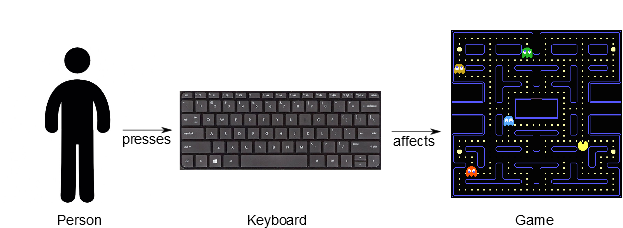
\includegraphics[width=10cm]{Concept1.png}
\caption{\emph{Overview of the interaction between a person and a computer game under conventional use}}
\label{fig: overview_basic_interaction}
\end{center}
\end{figure}

The developed application can be seen as an additional element between a person and the keyboard key for controlling a game. In short, the OmniPlay allows a person to virtually press a key by performing an gesture chosen by the physical therapist (see figure \ref{fig: overview_application_interaction}). This virtual key press is executed by the OmniPlay application, invoking the appropriate Windows operating system command. This invocation has the same effect as pressing the specified key on a physical keyboard. Further on, this action is referred to as pressing a virtual keyboard button. \\

\begin{figure}[H]
\begin{center}
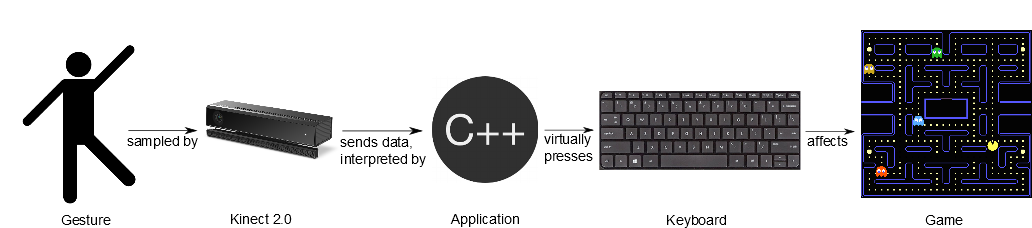
\includegraphics[width=14cm]{Concept2.png}
\caption{\emph{Overview of interaction between a person and a computer game using the developed application}}
\label{fig: overview_application_interaction}
\end{center}
\end{figure}

More in detail, the physical therapist comes up with gestures that fit the needs of a patient. He uses the Kinect camera to interact with the application via a GUI. Next, the therapist uses the application to record what gestures need to be done by the patient. Using all of the recorded gestures, an SVM model is created, which is used to predict which gesture is performed by the patient while playing a game.\\

The therapist assigns a virtual keyboard button to each of the gestures. This means that when the patient mimics one of the therapist's gestures, a virtual keyboard button is pressed, as explained before. To start playing a game, the therapist can choose any game or let the patient choose his preferred game. This can be any type of computer game and includes, but is not limited to: browser games, games that need to be downloaded and installed, pre-installed games that come with the operating system,\ldots If the OmniPlay is running in the background while a computer game is opened, performing a gesture indirectly presses the button that is linked to the gesture. By doing this, the patient can interact with the game.\\

By mapping gestures to virtual keyboard buttons, a vast amount of existing games can be played using gesture-based input. It is however limited to button presses. Pointing with the cursor like when using a mouse is not supported by the OmniPlay application. The reason is that every gesture performed is seen as one single action. The gesture of pointing to a specific spot on the screen could overlap with one of the gestures the therapist wants to use. This results in undesirable behavior and negatively impacts the gaming experience for the patient.\\


\subsection{Setup}

Before the application can be used, the user has to download and install the necessary drivers in order to use the Kinect 2.0 camera. To connect the Kinect 2.0 camera to a computer, an additional adapter is needed so it can be connected using a USB 3.0 port (see figure \ref{fig: kinect}). The use of the Kinect camera requires a socket. For using the Kinect, it is necessary to install a driver. This comes as part of the \emph{Kinect for Windows SDK 2.0}. Microsoft's download page \cite{KinectSDK} states the system requirements for using the Kinect 2.0 camera. These requirements include: a 64-bit processor, dual-core 3.1 GHz or faster processor, USB 3.0, 4 GB of RAM or more, graphics card that supports DirectX 11, Windows 8 or 8.1, Windows Embedded 8 or Windows 10.\\

\begin{figure}[H]
\begin{center}
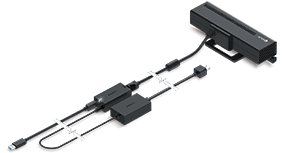
\includegraphics[width=8cm]{KinectAdapter.png}
\caption{\emph{The Kinect 2.0 camera connected to the adapter}}
\label{fig: kinect}
\end{center}
\end{figure}

The camera has to be placed horizontally in order to function correctly. The distance between the user and the camera may vary between 1.5 and 4 meters, depending on the height of the user and the size of the used screen (see figure \ref{fig: kinect_setup}). The camera can be tilted upwards or downwards. The chosen angle depends on the height of the camera. Both can be chosen freely by the user, but the user has to ensure that he is fully visible at the position he stands. The GUI allows him to verify this. A possible configuration that works well is to have to Kinect camera pointing straight ahead on a table with a height of approximately 0.8 meters.\\

\begin{figure}[H]
\begin{center}
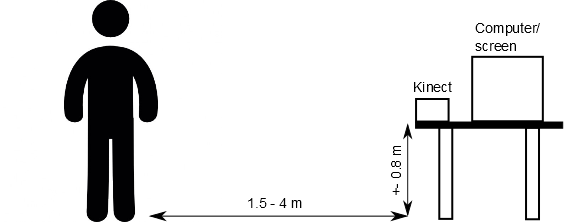
\includegraphics[width=12cm]{SetupKinect.png}
\caption{\emph{Setup for the Kinect camera}}
\label{fig: kinect_setup}
\end{center}
\end{figure}

%Before starting the application through means of an executable file, it is recommended to put this file in a directory that does not need to change over the course of multiple uses. The reason is that a subdirectory is created in the same directory, containing all data files of saved gestures. As long as this data folder and the executable are in the same directory, all previously recorded gestures are loaded when starting the application. If they get separated, the application still can be used, but it appears as if there are no saved gestures and it creates a new data folder in the directory the executable is stored.\\


\section{Graphical user interface}

A large part of this thesis was focused on the design and implementation of a user-friendly interface that can be controlled via input from the Kinect 3D camera. The reasoning behind this is that the user does not want to run back and forth from the standing position in front of the Kinect and the keyboard. Many interfaces have been designed for use with the Kinect but they are generally only used to get to the game and are therefore made up of standard WIMP elements (window, icon, menu, pointer) such as buttons and scrollbars to select your option. In this section, the process of developing the user interface and the properties of the coded prototype are discussed.\\

The goal in this part of the thesis is to find a new way of interacting with a user interface using the Kinect camera that feels natural to the average user. This despite the claims by Norman \cite{Norman2010} that natural user interfaces (NUI), the term that is often used to describe interfaces controlled with 3D cameras, are not natural because there is not the same feedback as when acting on objects in real life. Standard WIMP elements definitely do not feel natural in a NUI, pointing and clicking on buttons with a pointer may have already become second nature to modern humans, but it is a whole other thing when they are large and floating in the sky or fixed to a wall and the user has to slap them or close their fist over them without getting any inherent feedback as Wensveen \cite{Wensveen2004} called it. For this reason, elements such as push buttons, scrollbars and floating windows are avoided. Additional hardware is not desirable and voice control is also not considered because it is an area where plenty of research has been conducted already and implementing such an system is impossible considering the limited time for this project. If possible, we wanted to find new ideas on how to control a NUI.\\


\subsection{Hierarchical task analysis}

To figure out what steps the therapist needs to perform to use the program, a hierarchical task analysis (HTA) is performed. This is a process in which all necessary tasks and subtasks are put into order to get a sense of the properties and elements that the UI must possess. This started as a very technical plan of the tasks that are needed, but is quickly distilled into a simple visual plan that can be shown to the user to give them a good idea of what is required of them. This plan can be seen in figure \ref{HTA}.\\

\begin{figure}[H]
	\begin{center}
		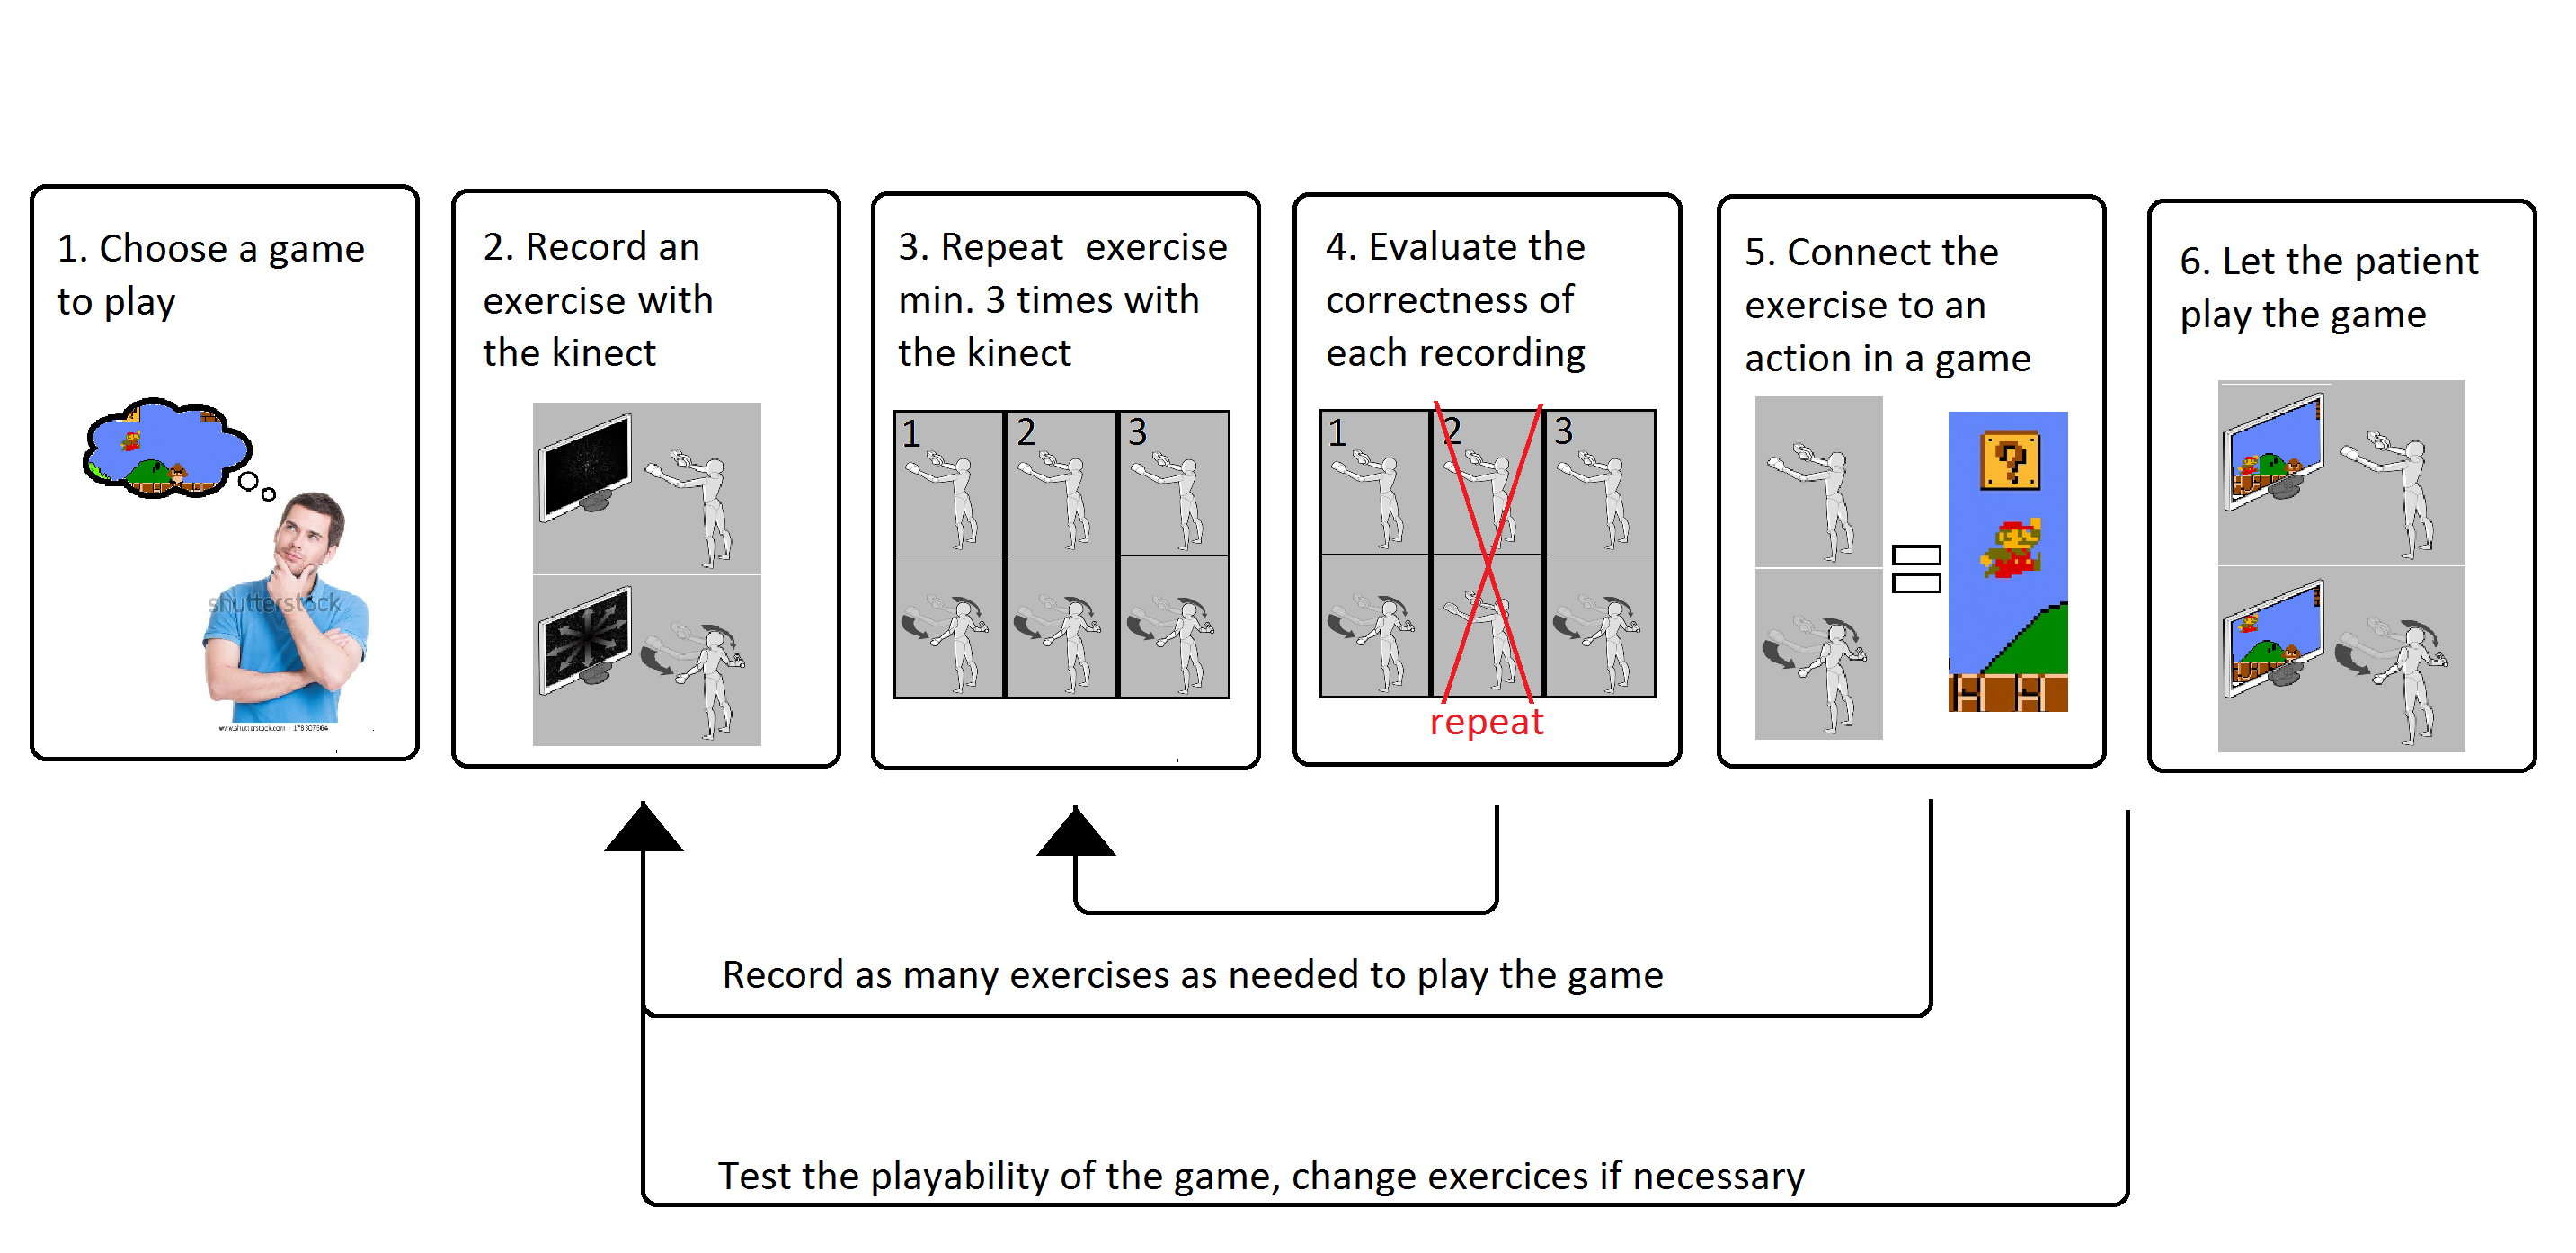
\includegraphics[width=14cm]{figures/HTA_plan.png}
		\caption{\emph{The simplified HTA plan}}
		\label{HTA}
	\end{center}
\end{figure}


\subsection{Experimental brainstorm technique}

A brainstorm session with the targeted user, the physical therapist, would give us fresh ideas on how the user expects to interact with a user interface using his body or voice. The expectation was that two distinct observations would be made: how the user wishes to interact with the user interface and how he expects the program to function.\\

% {\large COMMENT: is WIMP de juiste term in het vorige stuk? }
 %{\large COMMENT: hadden wij toen al dat visuele stappen plan? ik denk het niet he }

The idea is to prevent the subject from being influenced by our ideas or by obvious solutions. To start only the basic concept of our application and the abilities of the Kinect camera are explained. Then the subject is asked how he would imagine every expect of the application, a few questions from the script are: What information would you expect to see on the screen? How would you start a recording? What would you want to see during recording?\\

To find out whether such a brainstorm session would yield any viable results, brainstorm sessions with our relatives were conducted first. Two iterations were performed with four subjects, the first test was with two males and the second was with two females, of both genders there was one person around 25 years old and one around 55 years old. Each subject was interviewed completely separately to minimize the influence they had on each others ideas.\\

The sessions were very taxing for the test subjects, as the concept we tried to introduce was too abstract and foreign to them. This causes them to be shy with proposals, even after being ensured that there are no bad ideas. It seemed to give them the feeling that they are not smart enough to make good proposals. As a result they fell back on proposing  familiar UI elements or concepts such as push buttons or voice control. Getting locked into a mindset that we were designing games to play with the Kinect was also a minor issue, thereby answering the questions with that in mind, which was not the point. After two iterations with minor changes between them, we decided not to subject the physical therapist to this kind of questioning. Setting up a meeting would waste to much of his precious time with little gain to us. Worse, it might instill the physical therapist with a feeling of dread for our next meeting which might reduce his level of co-operation.\\

 %{\large COMMENT: hier mag we een of andere splitsing komen die duidelijk een onderscheid maakt tussen dees 2 delen}

Instead the decision was made to brainstorm with each other and our supervisor to develop a few prototypes that we can eventually show to the physical therapist to see which one seems the most user-friendly. The two mayor interaction patterns that came out of this brainstorm session are, for the purpose of this thesis, named the hints and mime patterns. In the rest of this chapter the abbreviation UI is used to say user interface and a UI element is a button, scrollbar or any other element that the user can interact with. When discussing the different concepts we often refer to a movement by the user or position that is taken to activate a function in the program as a sign.\\

The hints pattern implies that the screen is largely devoid of UI elements and actions are performed when the user does a certain movement or takes a certain position, for example, the user forms a cross with his arms to delete a recording. It is called the hints pattern because it is similar to how a game of hints is played. This is a game where one player tries to depict a concept or activity without using his voice, the other players have to guess what he is trying to say. In this case the user is the player who is depicting the concept or activity and the program needs to guess what the user means. There is a slight difference here in that the program already knows which signs the user can choose from. Though not always possible, it is better when a sign activates a function in the program that is similar to the concept or activity that this sign refers to in everyday life, as in the last example where an X is related to delete because it generally means bad, wrong or unwanted in Western culture, but this might be different for other cultures as Norman \cite{Norman2010} pointed out. The lack of feed forward that this implies means the user should learn all of the signs at the start of the application, putting a large strain on the user's cognitive ability which is not ideal. One could compare it to the shortcut keys on a keyboard such as CTRL+ALT+DEL. There is no indication on the UI that this key combination performs a special function. Norman \cite{Norman2010} made these complains and that is hard for the user to find out what he is doing wrong if he doesn't do the sign right. Alternatively, all possible action could be displayed on the screen around the user with a depiction of the sign. Though this would put less strain on the user's cognitive abilities, he would still have to focus on these pictures and try to figure out what sign they depict. But what if the sign is a movement? It is impossible to depict it statically, so how can you make this clear without distracting the user with constant moving pictures? A more significant problem might be the fact that positions and movements might be recognized by accident, an undo movement could partly solve this but you also need a redo button to compensate for any accidental undo-activations. The only real benefits to using the hints pattern is that activating an action can be done from anywhere and it could be faster once the user has mastered the signs, though this depends on the ease of performing the signs and the delay between a sign and the corresponding action in the program.\\

The mime pattern, as the name suggests, is the act of mimicking an action that is needed to act on everyday objects such as opening a door. But where an mime artist does this without any indication of that object being there, here an image of for example, the door would be displayed on the screen. The technical term for such a UI element is a metaphor because the function is similar to what a user would do with the object in real life. The power of this pattern is that the user should immediately recognize the UI element and know how to interact with it because it has the same affordances as the object in real life. To achieve the best effect, the UI elements that are chosen should need signs that the user has done frequently already, so that doing them feels natural and familiar. Linking a sign to a function that is similar to the use of that sign in real life, such as going to a different screen when opening the door, improves the interaction but it is less important than in the hints pattern. Wensveen \cite{Wensveen2004} already said that for this to work correctly feedback is crucial, the reaction of the UI element must match the expectations of the user otherwise he will be confused and the flow of the program is interrupted. Disadvantages are that the user cannot activate every action from anywhere and it might be slower because of that. Both Wensveen \cite{Wensveen2004} and Norman \cite{Norman2010} state that inherent feedback is lacking here, the user doesn't feel the UI element with which it is trying to interact. \\
%{\large COMMENT: look in notes HCI for extra idea's from the literate study }\\

One should prevent mixing the two patterns because the user expects to interact with everything on the screen when using the mime pattern, if one action is activated using the hints pattern without indication the user will be confused when he has forgotten the sign. Even if there is indication, the user will likely try to interact with the indicator of the sign as a button which will not have the desired effect. Combination with regular WIMP UI elements, such as push buttons or scrollbars, is possible for both patterns, but it combines much better with the mime pattern since the user is already interacting with elements on the UI while pointing at a specific area in the UI doesn't fit well in the concept of the hints pattern and would even detract from the idea of being able to do every action everywhere. To sum up, in the mime pattern the behavior of the UI elements are simple and obvious but possibly more inefficient, like pulling a handle on a slot machine to spin the slots. While the hints pattern is more abstract and complex, but should allow a more efficient interaction once mastered.\\


\subsection{Prototypes}

With these patterns in mind the design of the prototypes focuses more on designing UI elements and methods with which the user can interact that are simple, fast, ergonomic, feels natural and is not taxing to the user physically or cognitively while being practical and not easy to activate accidentally. The regular way of testing a concept UI is by doing paper prototyping which means that the user is presented with a paper version of the UI (hence the name), whenever the user touches a UI element the designer manually changes the paper prototype to reflect the activated action. This kind of testing is absolutely not suited for the goal of this project, it is more to assess the placement and shape of UI elements and the general flow of a program. What is needed here is a way to interact with the prototypes in a way similar to how the real program would work but without having to code the whole program. For that reason we took two example programs from Microsoft's Kinect SDK and made some adjustment to show the user in front of the prototype.\\

When designing a motion controlled UI it is very important to let the user know what the camera sees of their signs. The manner in which this feedback is given will have a great impact on how natural the user's experience with the UI will be. There are four viable options:\\

 1. A real image of the person as the camera films it (figure \ref{user visualizations} a).\\
 2. A semi-transparent schadow of the user (figure \ref{user visualizations} b).\\
 3. A puppet that copies the user's movement (figure \ref{user visualizations} c).\\
 4. No body is shown, only images that portray the position and state of the hands (figure \ref{user visualizations} d).\\
 
 \begin{figure}[H]
 	\begin{center}
 		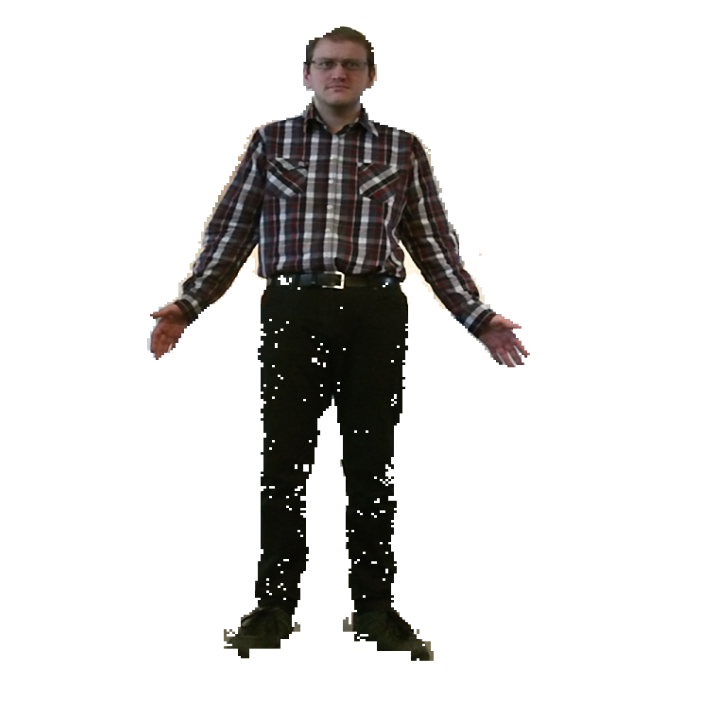
\includegraphics[width=7cm, height=7cm]{figures/real_image_example.png}
 		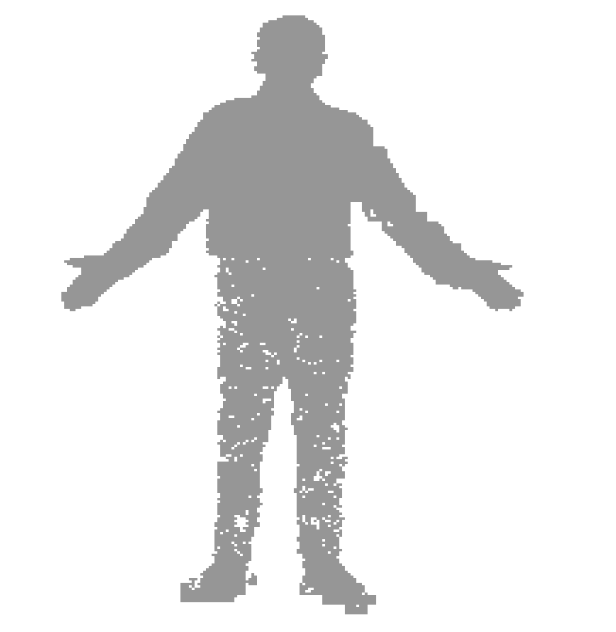
\includegraphics[width=7cm, height=7cm]{figures/schadow_example.png}
 		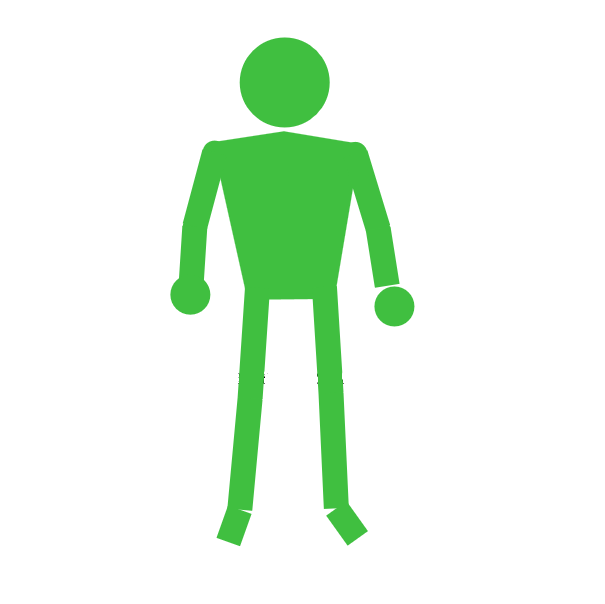
\includegraphics[width=7cm, height=7cm]{figures/puppet_example.png}
 		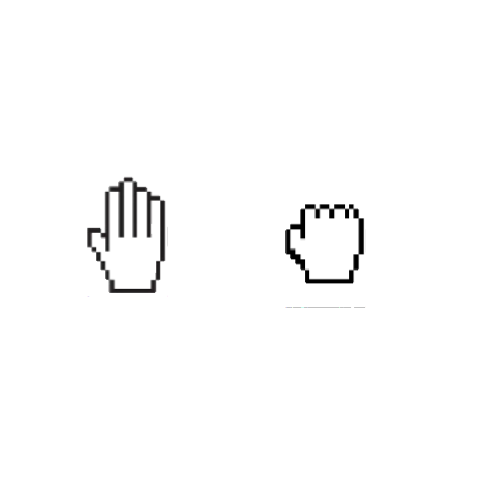
\includegraphics[width=7cm, height=7cm]{figures/hand_example.png}
 		\caption{\emph{(top-left) a: the UI with a real image of the user, (top-right) b: the UI with a semi-transparent shadow, (bottom-left) c: the UI with a puppet, (bottom-right) d: the UI with only hands visible. }}
 		\label{user visualizations}
 	\end{center}
 \end{figure}
 
 
A real image of the person is the most identifiable for the user because it is literally an image of himself, but this doesn't mean that it would be the best option to use in interacting with the UI. Though it has the advantage that it is crystal clear which movement the user carried out, which is good for recording and replaying gestures. The most important issue is that the image is taken from the front so the image of the screen is facing away, so unless the UI elements are drawn on top of the user's image it is hard to imagine you are grabbing a handle or pushing a button on the UI. Placing the Kinect camera behind the user to solve this problem, is technically not possible because an important part of the Kinect's person recognition is based on recognition of the facial features. This would also require a very large amount of room to operate because a distance of at least a one meter from the screen in front of the user and at least 1.5 m from the Kinect at the back needs to be maintained. When the UI elements are drawn behind the user, he will also obscure any elements directly behind him. Another issue that became apparent during the user tests was that most people are not comfortable with an image of themselves being displayed on the screen, which could detract from the user's experience. The physical therapist we interviewed, who works in a school for disabled children, also noted that this might cause legal problems with parents who do not want unauthorized footage of their child being stored. A final technical issue is that displaying the real image of the user is very resource intensive and in this implementation it would sometimes cause the program to lag.\\
 %{\large COMMENT: Why can't the real image also be transparent?}\\
 
A semi-transparent shadow would solve the legal issue, the discomfort experienced by users and it also solves the problem of the image facing away from the UI because there are almost no features that indicate which way the image is facing, making it look like the shadow is facing towards the UI. By making the image semi-transparent any UI element behind the user can still be seen. A disadvantage is that it is harder to identify subtle differences between similar recordings. It is also still very resource intensive, trying to optimize this was beyond the scope of this thesis.\\
 
A puppet that copies the movements of the user has similar benefits to the shadow and can be transparent or non-transparent. It is far less resource intensive but makes it even harder to distinguish similar recordings from each other.\\
 
Showing no body and only hands can obviously only be used to interact with the UI and not for the recording of a gesture. It removes all distractions from the screen and shows only the information that is essential for the user to interact with the UI. But because of this the interaction might feel less natural to the user.\\
 
The shadow type of representation has the most advantages so it is chosen to make the most prototypes with. Though the more abstract prototypes use the representation that only shows images of the hands of the user to see whether a more abstract representation really detracts from the user experience. \\
 
In this thesis three prototypes are discussed ranging from obvious UIs using mostly mime pattern elements and metaphors to more abstract UIs where more elements of the hints pattern and standard WIMP concepts are used with less mime pattern elements. The first two prototypes are only the screen in which the user can record one gesture multiple times to provide the data for the SVM (step 2 to 4 in figure \ref{HTA}). They use a shadow image of the user to control the UI. The other prototype is a menu to browse to a recording and replay it while the user only sees images of his hands (see figure \ref{HTA}). There are also other prototypes but only these three are discussed to show the kind of elements that were experimented with, these can be ordered as following:\\

1. A UI with mostly mime pattern elements and metaphors.\\
2. A UI that combines mime patterns with WIMP elements.\\
3. A UI that combines the hints pattern with WIMP elements.\\

The first paper prototype, that can be seen in figure \ref{first prototype}, mostly uses the mime pattern and metaphors. The orange color is used to indicate a possibility for an action. On the right the door on the side says exit and would swing open when the user grabs the orange handle an pulls to the left. On the top of the screen a collection of recordings can be seen pinned to a scrollbar with orange thumbnails. The arrows on the sides imply that the recordings can be moved. The user would grab the orange indicator bar to browse the recordings. To delete a recording the thumbnail of that specific recording can be grabbed and dragged to the recycle bin to release it there. The user can display the recording by dragging it to the projector on the left side of the screen which would display the recording on the projector screen where the large "1" is displayed. In the middle, a camera with its lens pointed towards the user is displayed, by moving his hand forward on the ``opnemen'' button the user could start a recording.\\

\begin{figure}[H]
	\begin{center}
		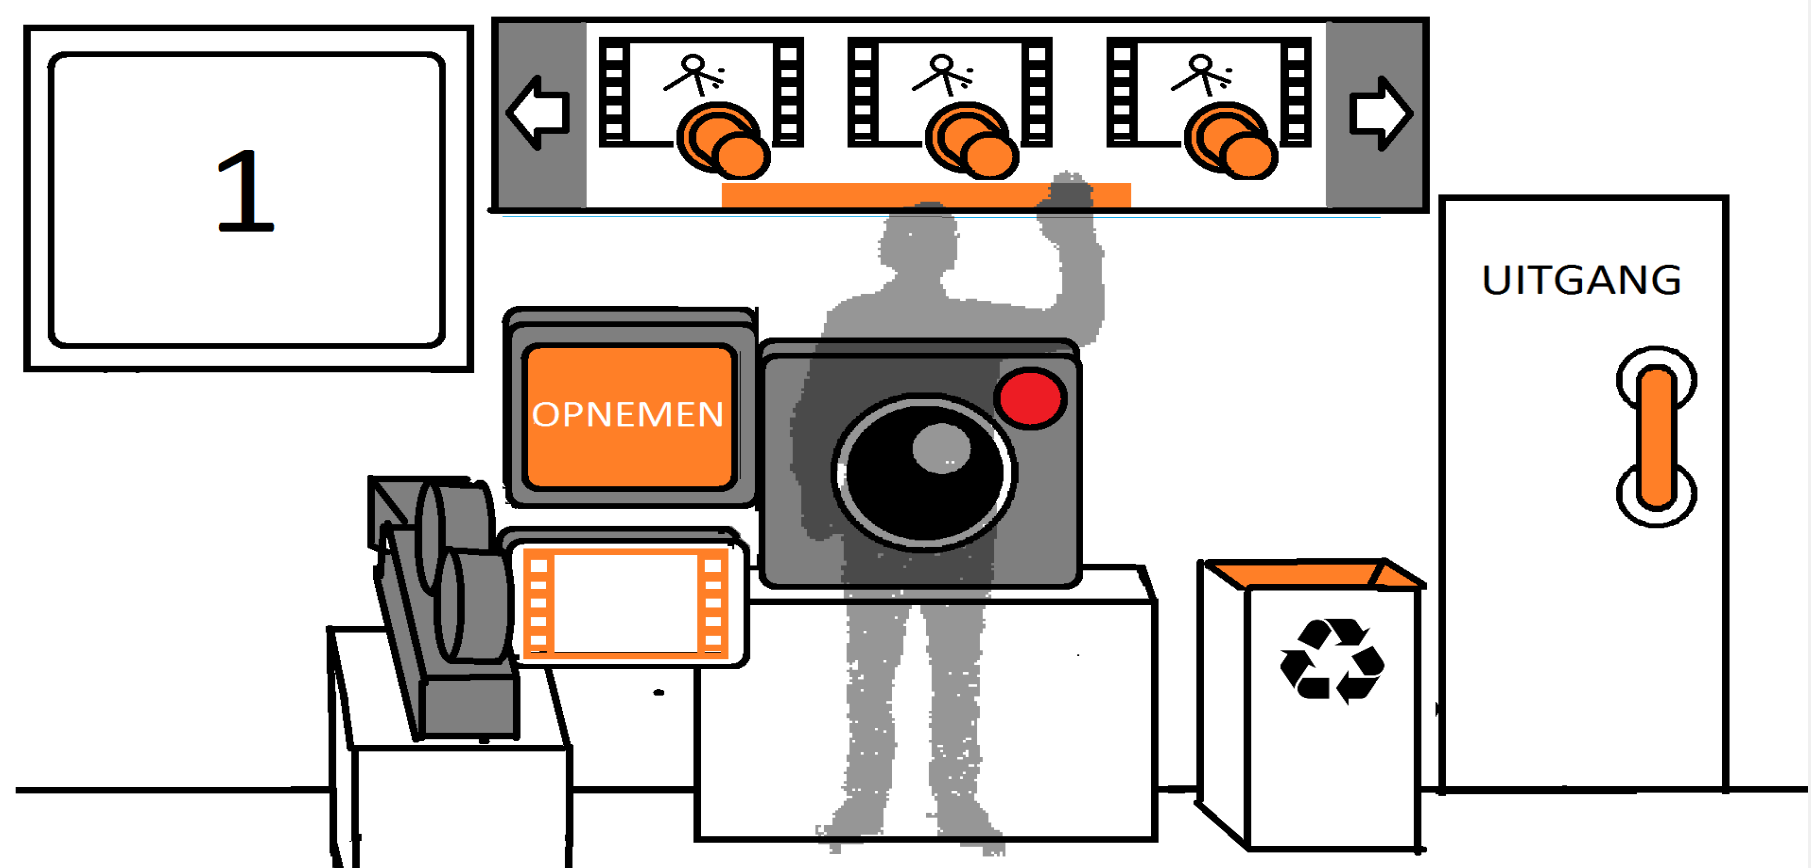
\includegraphics[width=12.5cm, height=7cm]{figures/prototype_1_1_standard.png}
		\caption{\emph{The first prototype screen}}
		\label{first prototype}
	\end{center}
\end{figure}

The second paper prototype in the list combines mime pattern elements with standard WIMP elements to streamline the process, it can be seen in figure \ref{standard third prototype}. On the right of the screen is a lever that is activated by grabbing the orange part of the lever and pulling it downwards causing the user the leave this screen. The record button is a push button that the user activates by moving his hand forward over it. This action activates the record screen as seen in figure \ref{record third prototype}. The window shows what is going to be recorded, the red one indicates where the program will count down from three until the recording starts, allowing the user some time to get to his starting position. All other UI elements are grayed out to indicate that they are not available to interact with. Once the recording is finished the program returns to the screen in figure \ref{standard third prototype}. On the left is a scrollbar that contains elements which represent previous recordings of which they show static representations. On the right of it, there is an orange scroll wheel with which the user can scroll through the scrollbar by simply hovering his hand over it. When the user stops scrolling the elements are locked into a position as it is shown in \ref{standard third prototype}. The user can slide the top element into the ``TRASH'' or ``PLAY'' area by hovering over it in that direction to play or delete the element.\\

\begin{figure}[H]
	\begin{center}
		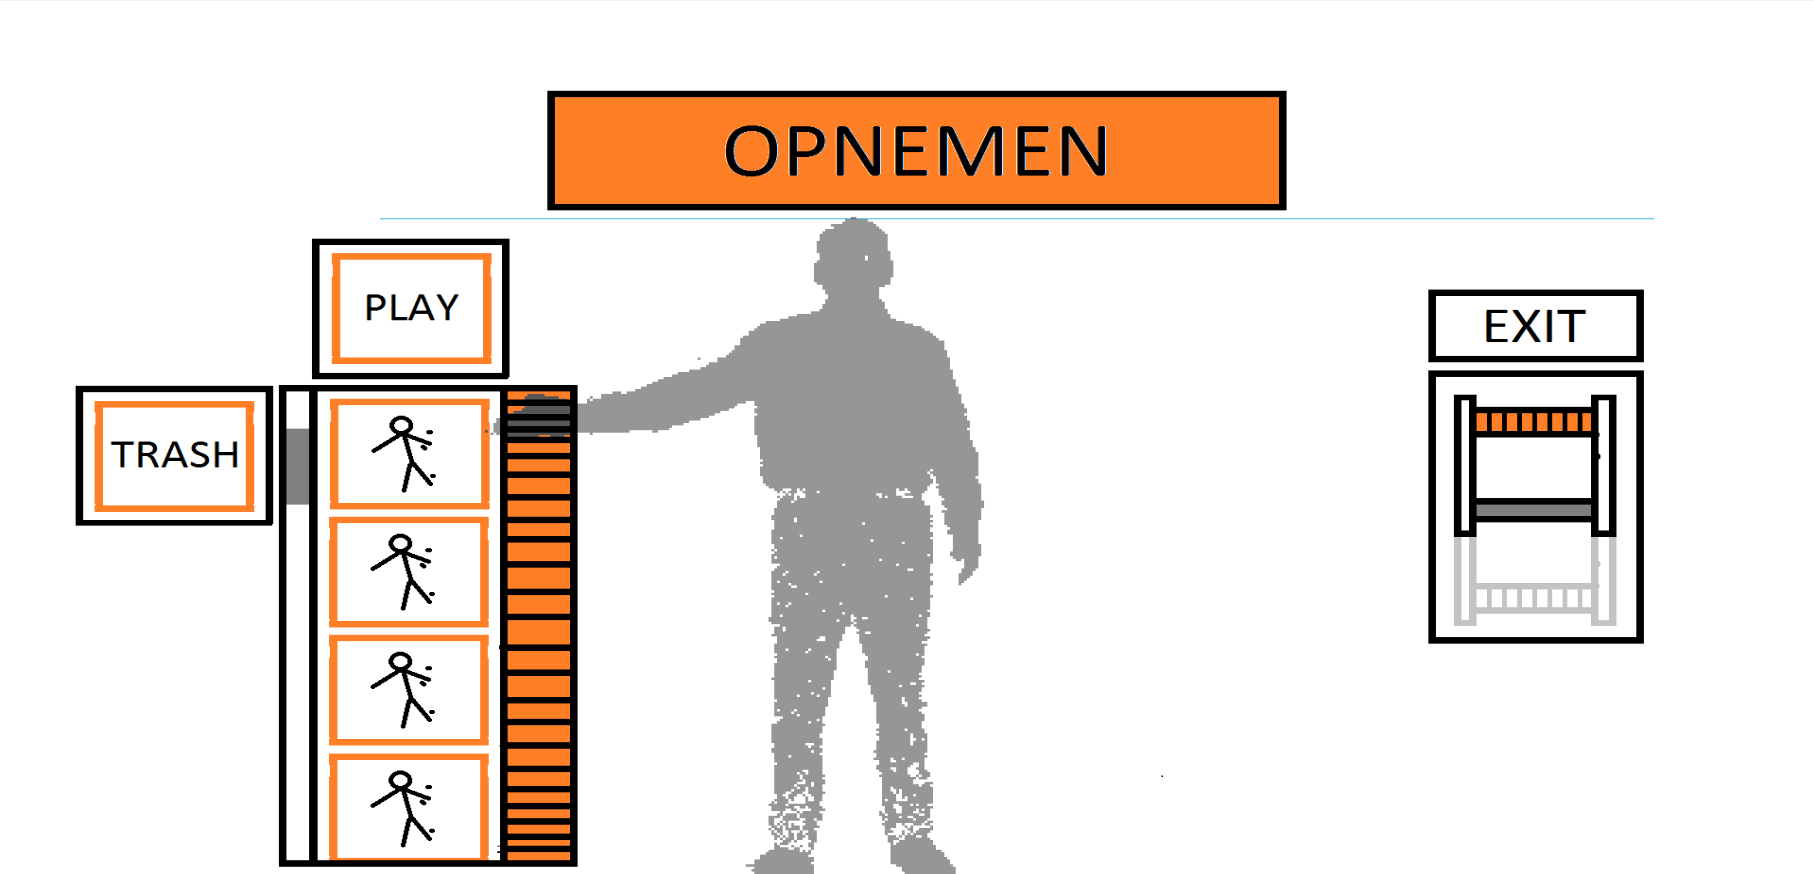
\includegraphics[width=12.5cm, height=7cm]{figures/prototype_5_3_standard.png}
		\caption{\emph{The standard screen of the third paper prototype}}
		\label{standard third prototype}
	\end{center}
\end{figure}

\begin{figure}[H]
	\begin{center}
		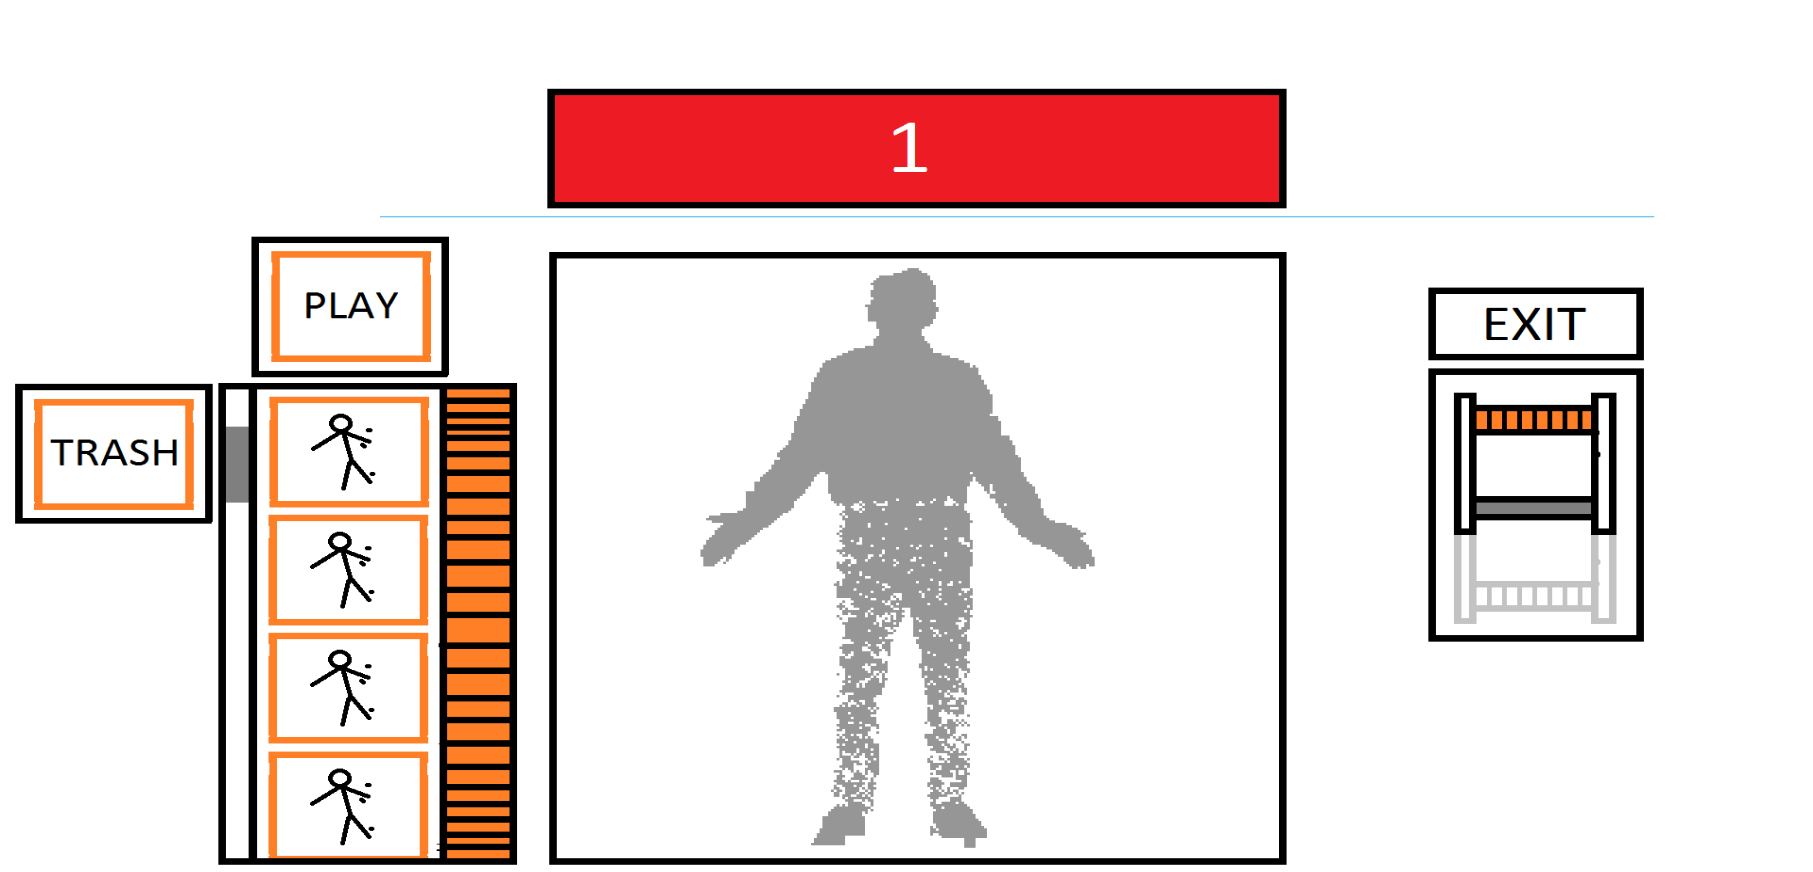
\includegraphics[width=12.5cm, height=7cm]{figures/prototype_6_3_record.png}
		\caption{\emph{The record screen of the third paper prototype}}
		\label{record third prototype}
	\end{center}
\end{figure}

The third prototype is a combination of the hints pattern where the user has to close his hand over the element with which he wants to interact to open a typical WIMP element called a context menu with which the user can interact. The user can only see images of his hands as discussed earlier in this chapter. It starts off with a small tutorial screen as seen in figure \ref{first tutorial last prototype}, when the user closes his hand within the orange box, the context menu as seen in figure \ref{second tutorial last prototype} opens. When the user slides his closed fist towards any of the elements it reacts as seen in figure \ref{third tutorial last prototype} to indicate the option is chosen. Throughout the prototype the user can interact with the chosen recording as seen in figure \ref{example last prototype}, in this instance he can choose between playing the recording, deleting it or canceling the current menu.\\

\begin{figure}[H]
	\begin{center}
		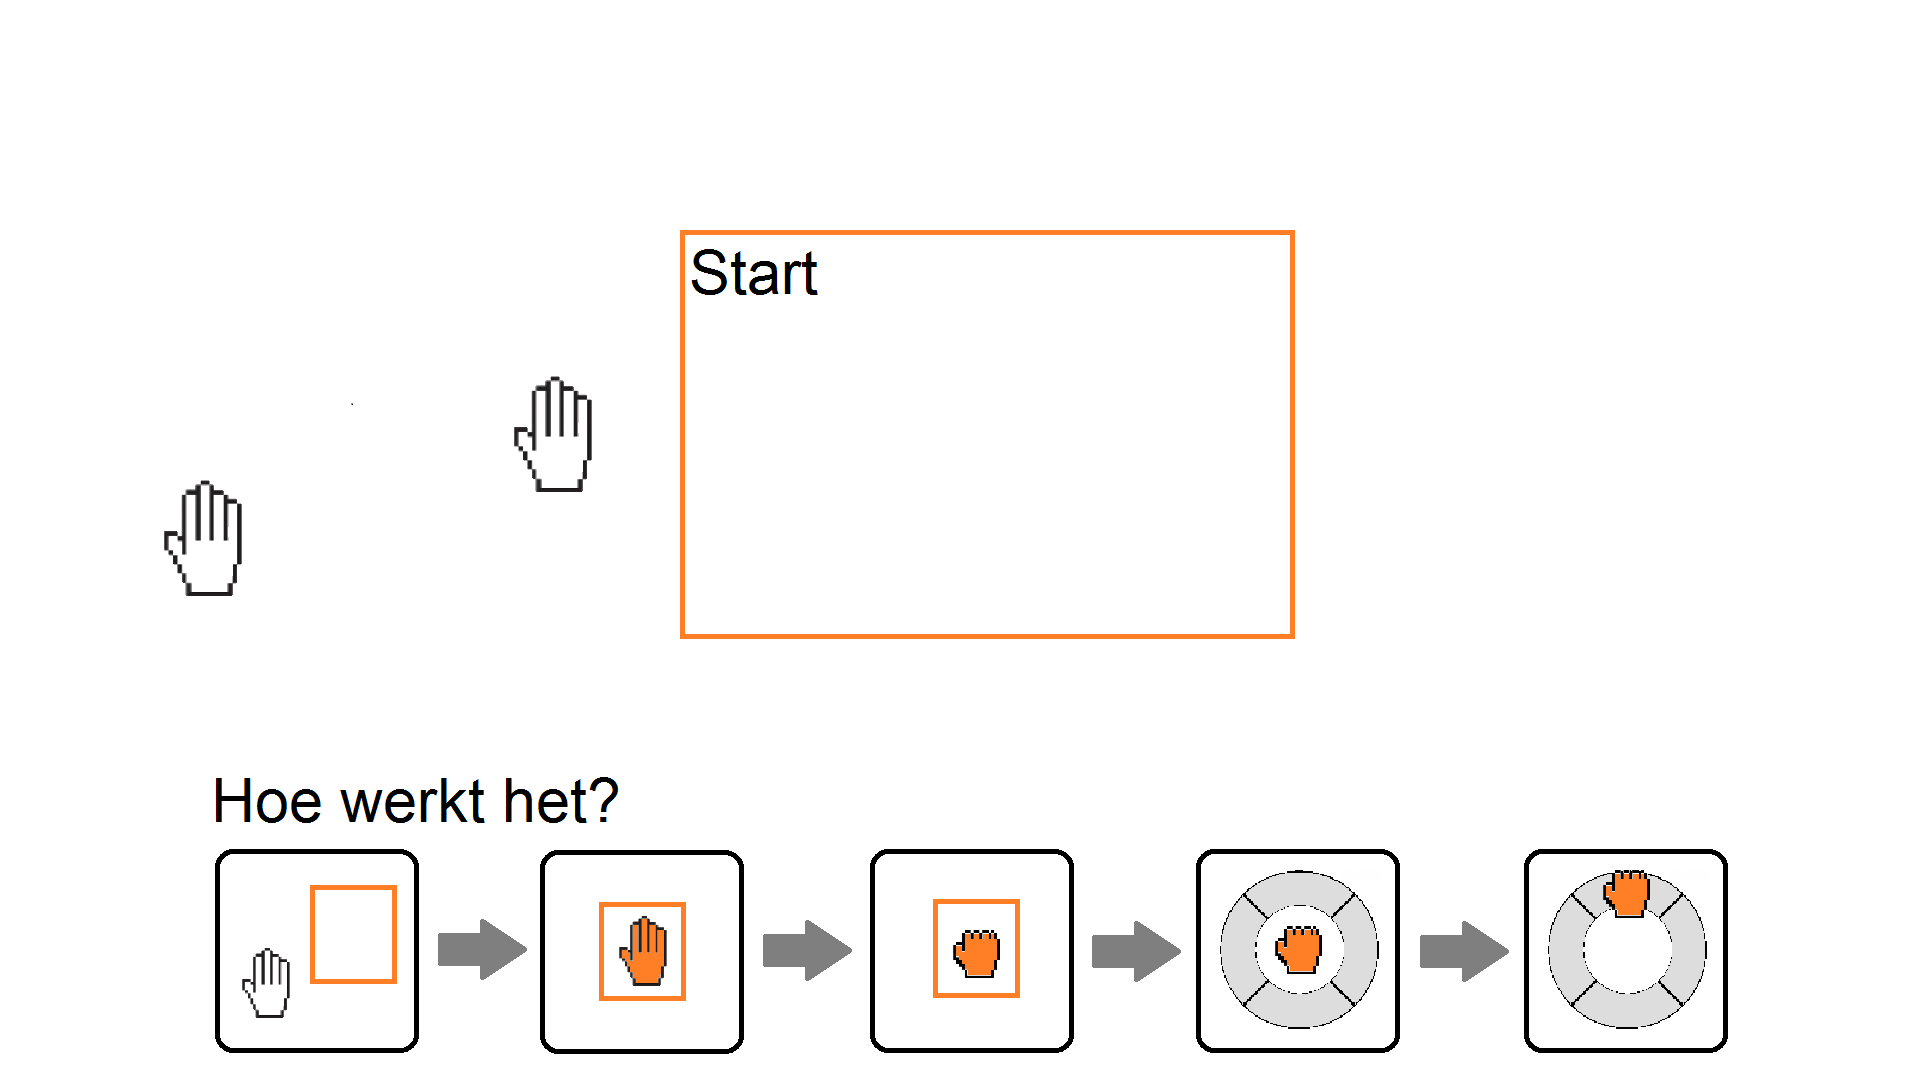
\includegraphics[width=12cm, height=6.5cm]{figures/prototype_7_6_tutorial_1.png}
		\caption{\emph{The first tutorial screen of the last paper prototype}}
		\label{first tutorial last prototype}
	\end{center}
\end{figure}

\begin{figure}[H]
	\begin{center}
		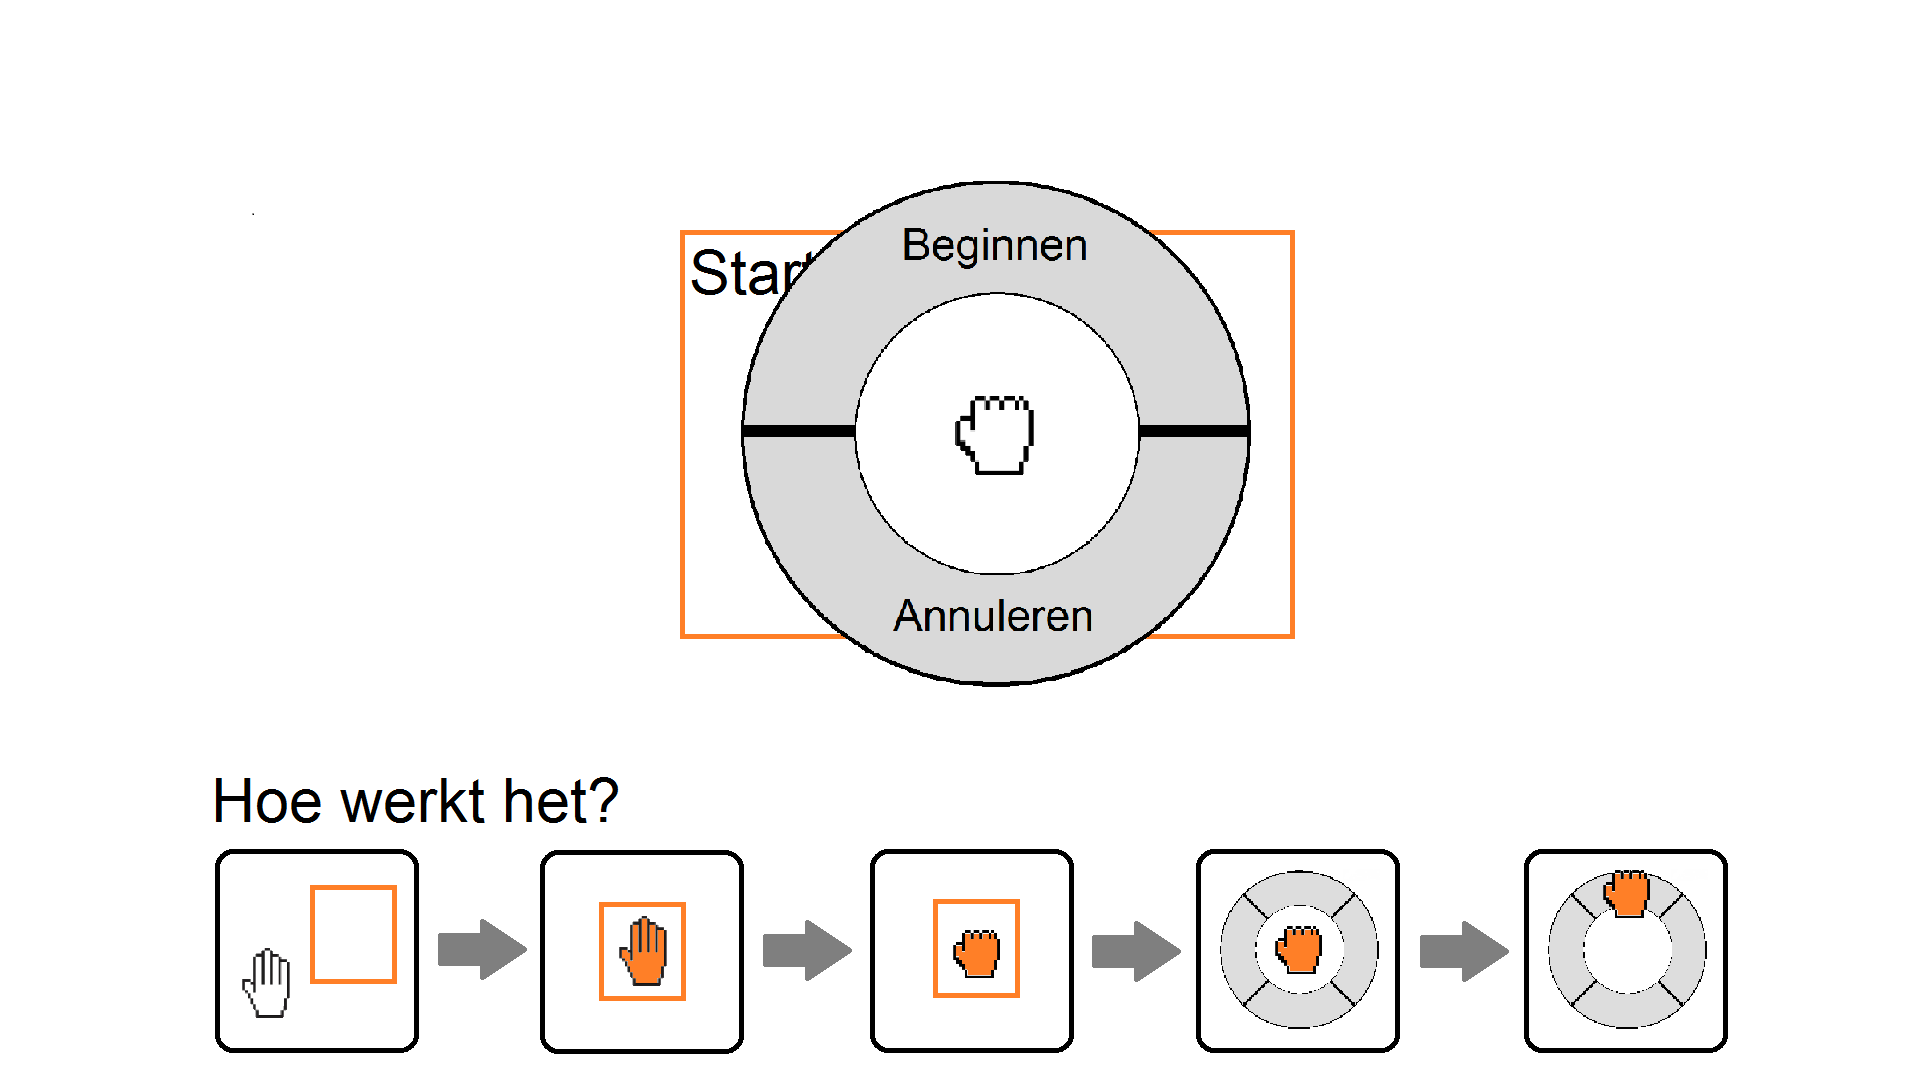
\includegraphics[width=12cm, height=6.5cm]{figures/prototype_8_6_tutorial_2.png}
		\caption{\emph{The second tutorial screen of the last paper prototype}}
		\label{second tutorial last prototype}
	\end{center}
\end{figure}

\begin{figure}[H]
	\begin{center}
		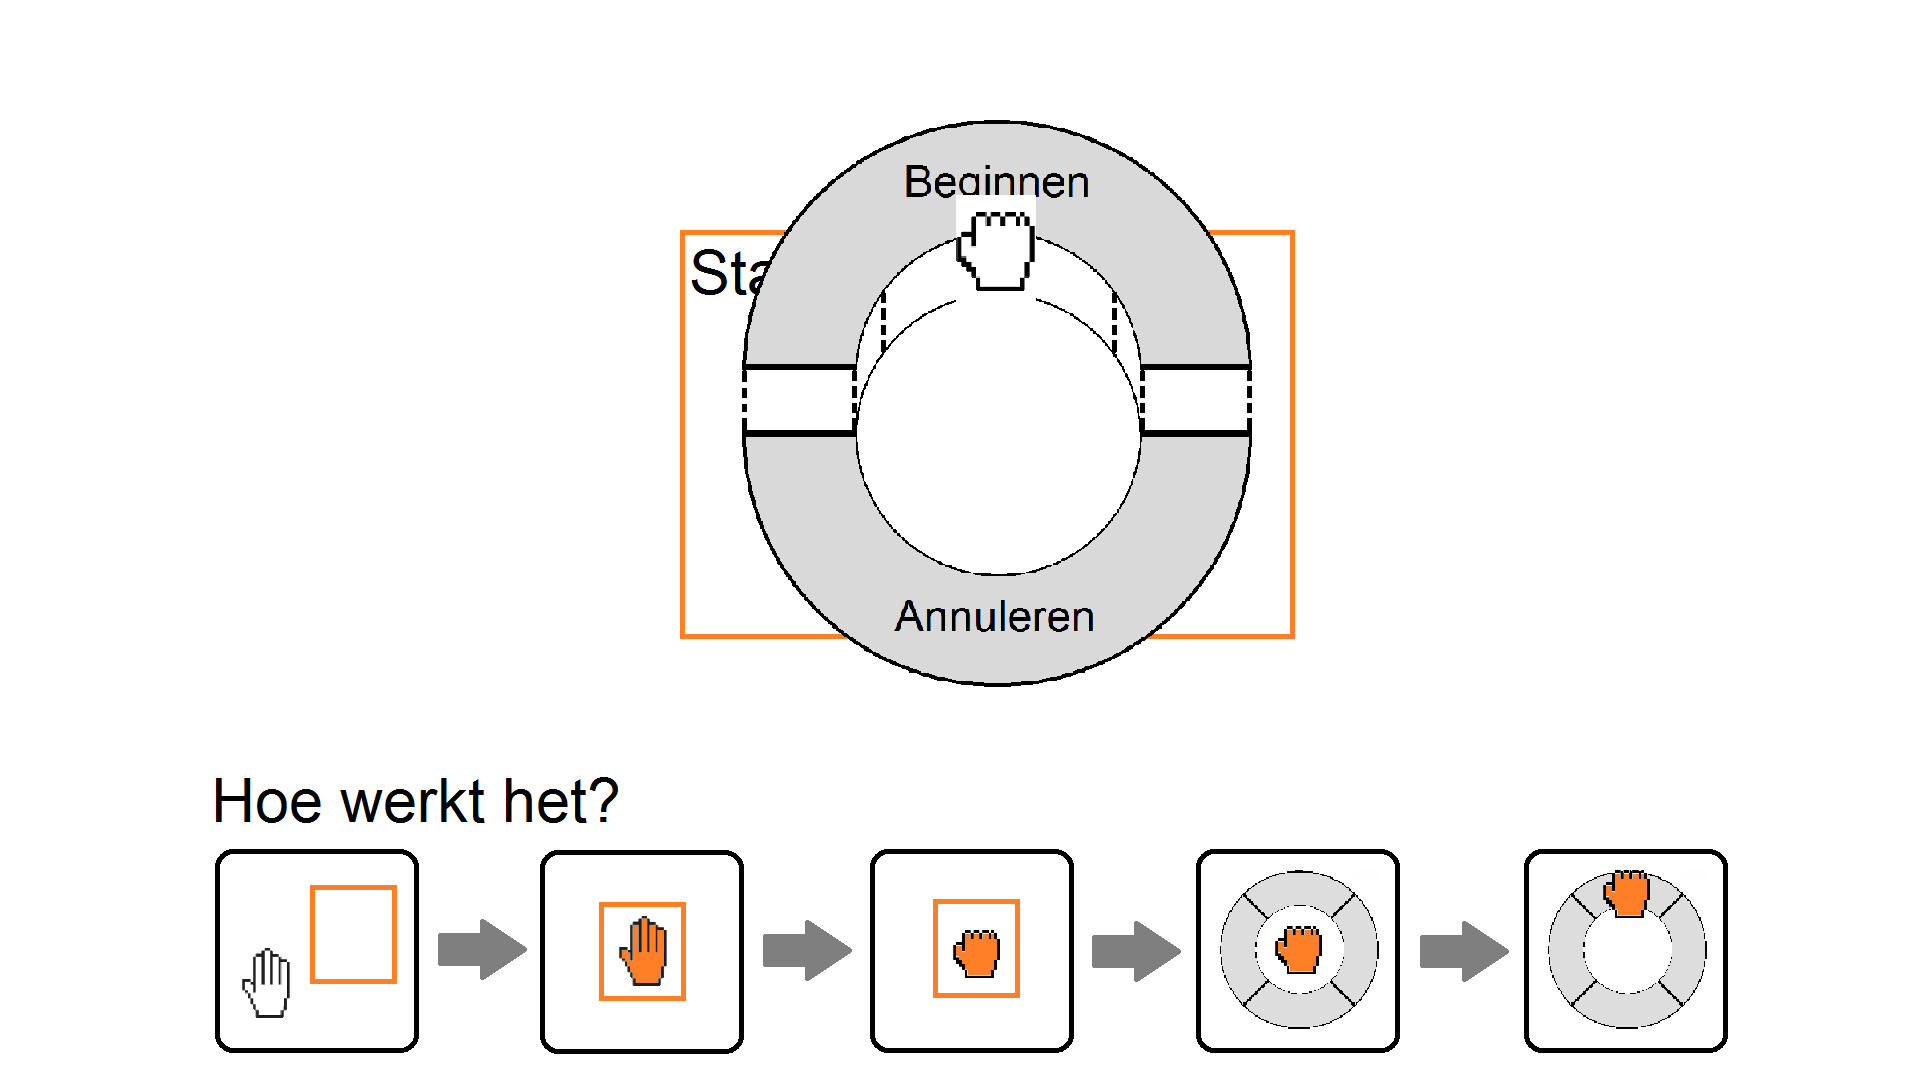
\includegraphics[width=12cm, height=6.5cm]{figures/prototype_9_6_tutorial_3.png}
		\caption{\emph{The third tutorial screen of the last paper prototype}}
		\label{third tutorial last prototype}
	\end{center}
\end{figure}

\begin{figure}[H]
	\begin{center}
		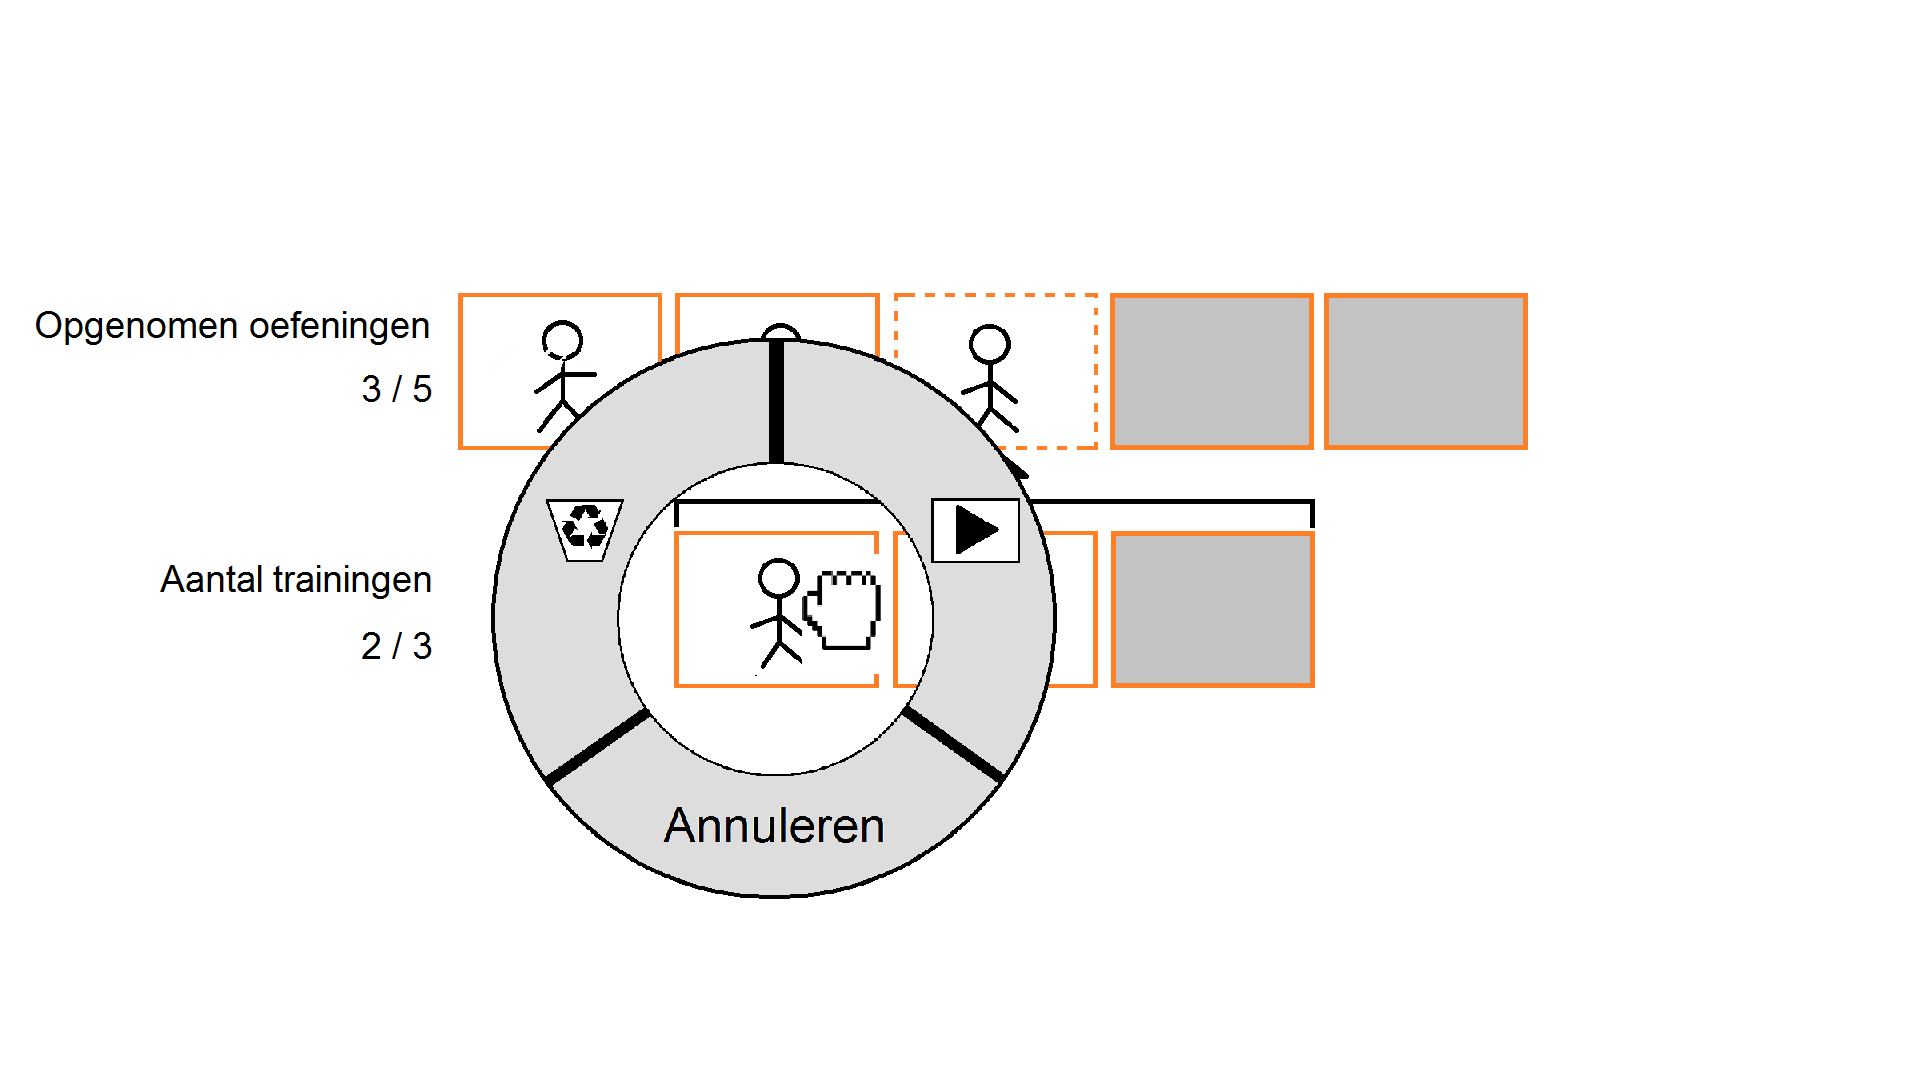
\includegraphics[width=12cm, height=6.5cm]{figures/prototype_10_6_example.png}
		\caption{\emph{An example of how the user would interact with and element of the last paper prototype}}
		\label{example last prototype}
	\end{center}
\end{figure}


\subsection{Prototype user test}

The main goal of this user test is to see how the user interacts with the different paper prototypes, how fast can he do the required signs and his opinion of the signs, whether they feel natural or not and which one of the paper prototypes is favored by the user. \\

For these tests, the Kinect is placed on a table of regular height and the user is asked to stay within two to four meters distance from the camera. The screen with the UI is placed directly behind the Kinect camera.\\

The user is first introduced to the concept and flow of our program through the use of the HTA plan as seen in \ref{HTA}, to bring the user up to speed with what is necessary to operate the eventual program. Then a small demo program is presented showing the capabilities of the concept and the Kinect to give him an idea of the end goal and the possibilities with this concept. After some more introductory questions the user is assured that he is never at fault and that we are responsible for any misunderstandings he might have. Before the actual tests, permission is asked to film their proceedings. During the tests the user is reminded that we like to hear his thoughts on what he sees and thinks.\\

Then the user is asked to interact with the prototypes using the Kinect. To mimic the functions of the UI, a variation of the Wizard of Oz method \cite{WizardOfOz} is used to change the screens whenever the user performs the required action. Some prototypes still require some explanation but generally the user is only assisted when he is completely stuck and at the end of every prototype an explanation of the intent of each UI element is given. At the end every prototype is gone over again without the Kinect to reflect about the performance of every prototype. The user is asked to select a personal favorite.\\

In total four candidates were subjected to these tests of which were one physical therapist and three relatives or friends but this paragraph will focus on the results with the physical therapist supplemented with the results of the others, thereby the physical therapist is referred to as \emph{the user} and the others as \emph{the other users}. It is important to mention that the user has previous, albeit limited, experience with Kinect games which sometimes influenced his reaction. For instance, he did not know that he could move his hand forward to mimic pushing a button because in his previous experiences this is never used. For the first prototype \ref{first prototype}, the user was trying to interact with UI elements that were not intended to be interacted with, he later indicated that he did not see the metaphors as they were intended, the screen was too hectic and he didn't see which ones were buttons and which were not. He also found that some signs required him to reach too far. Most of the other users also made the same remarks about the first prototype. A rope in one of the prototypes on which the user could pull was clear to him, but he had no idea how to interact with the scroll wheel to scroll through the scrollbar. In one of the prototypes the screen changed based on where the user was positioned, this caused a great deal of confusion, the same goes for the other users. The lever on the third prototype as discussed above, to leave the screen was clear but he did not like it, the metaphor was too foreign to him. The user was quick to pick up the controls of the last two prototypes that only showed the hands, but he later indicated that the representation of the hands only didn't feel right to him and that he much preferred to see all his options on the screen. Other users indicated that they expected the UI to react as if it were a touchscreen. When asked how they preferred to see the themselves on the screen, all users experienced discomfort with the real image of themselves and the therapist made the comment about legal issues with the patient as seen before in the discussion of the user's representation. They all preferred the shadow representation.  Remarkable was that all the users chose the third prototype, as seen in figure \ref{standard third prototype} earlier on, as their favorite, mostly due to the simplicity and clearness of it.\\

The conclusions are that the most important characteristics are that the screen needs to be simple and straightforward with all of the options displayed on the screen permanently and modes dependent on subtle parameters, such as the user's position, need to be avoided. The preferred representation of themselves is the shadow. For the purpose of simplifying the UI, regular WIMP elements are still allowed to be used without interfering with the user experience, though clearer affordances for elements that do not look like any object in real life are needed.\\


\subsection{Description of the interface}

The end design looks as seen in figure \ref{regular view end design}. Starting from the left, the user can see a gray window in which a recording can be replayed, this is a typical WIMP element because it does not have any elements to it that can be seen as a metaphor to anything the user is familiar with in real life. Right of this there is the rope, which is a very distinct mime pattern element. Further right is a simplified version of the scrollbar containing the recordings with the currently selected recording highlighted in orange. The user can slide this element to the "DEL" bar to delete the element. The black bordered box at the feet of the puppet represent the ground on which the puppet walks so it does not appear to float in mid air.

Though we had previously established that the shadow was the most natural way of representing a user in the interface, performance issues forced us to resort to using the puppet image. The reason why the puppet is not semi-transparent is because then the joints are more visible than the rest because two semi-transparent images are drawn on top of each other which combine into a less transparent color. This breaks the unison of the puppet's coloring making it seem less human which would be a distraction that detracts from the experience of the user. Another detail of the puppet is that the centerpoint of the spine is fixed in the vertical direction but not in the horizontal direction. This eliminates any dependency on the position of the camera so that, as long as the user is within the field of vision of the Kinect, he can always reach every UI element on the screen. This measure introduces two  problems. The biggest problem is that when the user tries to squat the puppet will lift its feet instead of lowering its torso, this might cause confusion and does not feel natural. The other problem is that the user cannot reach any UI element that is placed where it could only be reached by bending downwards. This is not seen as a big problem because such a sign is very taxing for an adult to perform and thus not wise to use in a UI. The puppet is free to move in the horizontal direction but there is an offset on where the puppet is drawn so that the puppet appears to stand between the rope and the scrollbar when the user is standing right in front of the Kinect. In a normal setup the screen will stand behind the Kinect so that the user can look straight ahead when interacting with the UI. The depth coordinates in 3D space are also set to a fixed distance before conversion to a 2D screen to ensure that the puppet is always drawn to the same size no matter how far the user is standing within the field of vision.\\

\begin{figure}[H]
	\begin{center}
		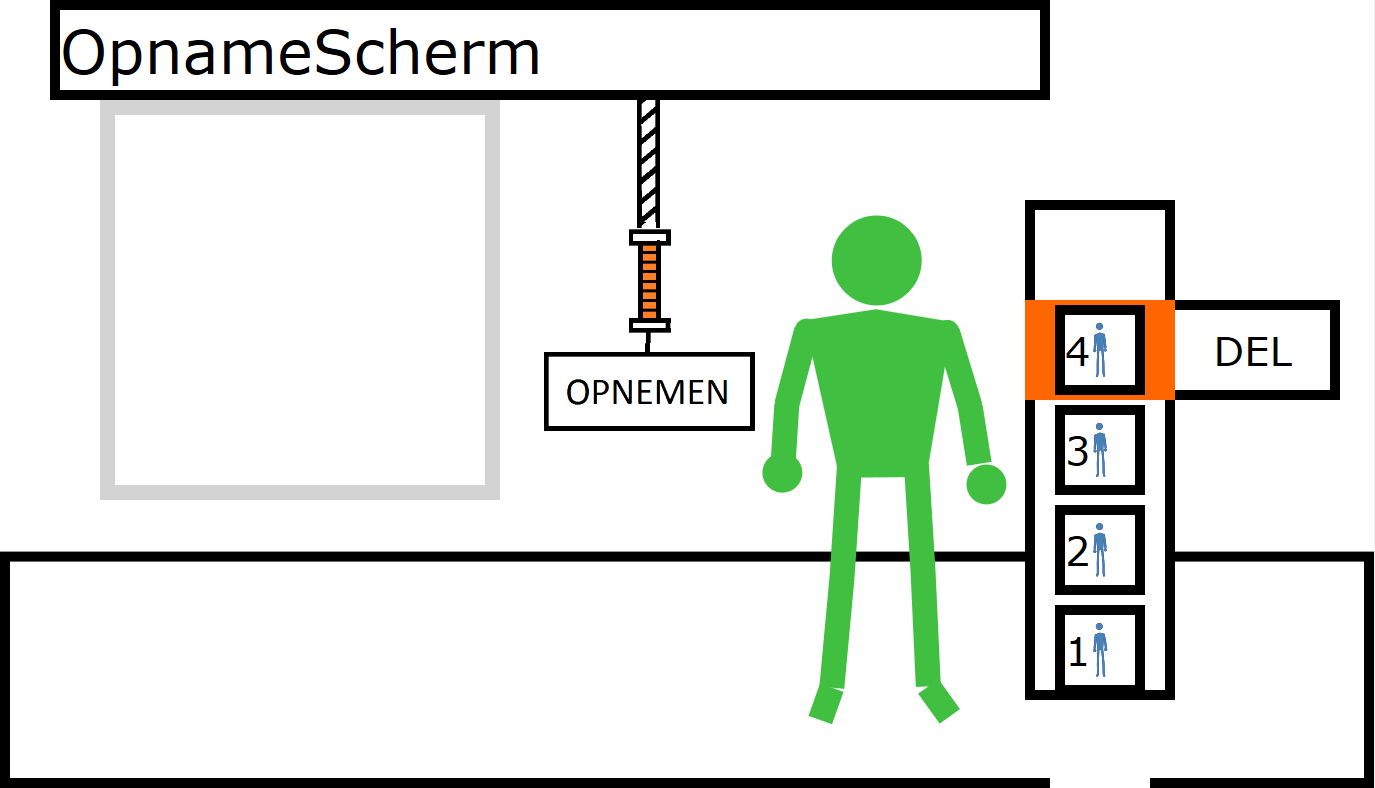
\includegraphics[width=12.5cm, height=7cm]{figures/1_screen_with_user.png}
		\caption{\emph{The regular view of the end design of the UI}}
		\label{regular view end design}
	\end{center}
\end{figure}

An important aspect of the UI is the color coding that is consistent throughout the UI except on the puppet itself though it should be apparent that the puppet is not much more than a representation of the user. This should give the user extra feed forward about what the consequence of his action will be. Orange is indication of interaction possibilities, green means a hand is hovering over the element, blue gives information about what happened or will happen after an action and red indicates a more serious action is about to be activated. The exact meaning of all these color codes will become clear during the description of the UI.\\

Since it is important for the user to know when the system sees that it is grabbing the rope, the UI provides feedback to the user by coloring the hands green when they are open and red when the user makes a fist.\\

In figure \ref{rope handle reaction} A can be seen that when the user hovers his hand over the orange handle of the rope the handle turns green indicating that it can now be grabbed. When the user closes his hand, the handle turns red to show the user that he is pulling it is shown in figure \ref{rope handle reaction} B. The dynamics for pulling the rope are simple, between the starting position and the end position, which is below the starting point, the rope will make the same relative movements in the vertical direction as the user makes with the center of his hand. In this way the interaction is linked in time, speed, direction, dynamics and location of the user's hand. When the rope is near to his end position the record screen is activated. There is no progress bar to indicate how far the user is from activating the function because generally the action of pulling a rope is very sudden and fast, as long as the function is activated before the user runs out of momentum this kind of feedback is not needed here. In the normal state the handle guards are not colored because the affordance is clear enough and a person would not normally grab a handle by the handle guards, they are however colored green and red to make it more apparent to the user that they are acting on it.\\

\begin{figure}[H]
	\begin{center}
		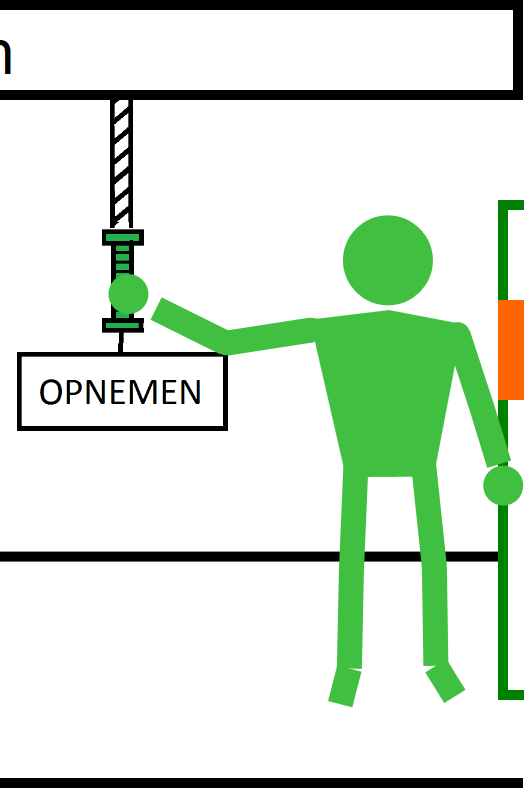
\includegraphics[width=6cm, height=8cm]{figures/2_hover_over_rope.png}
		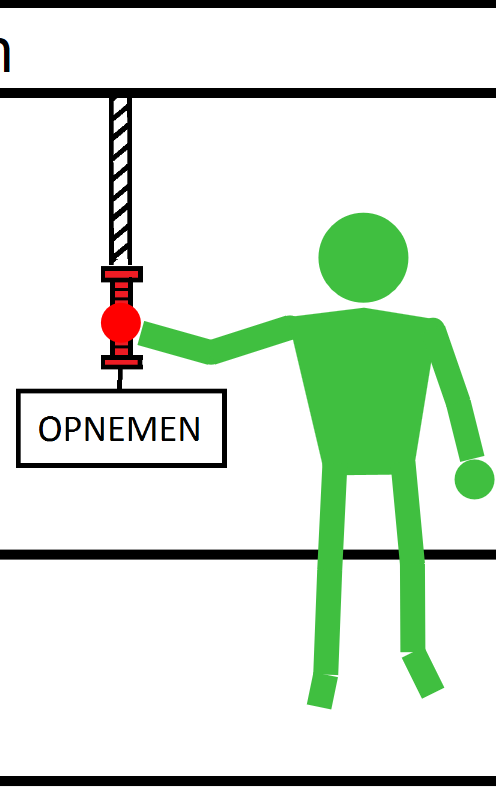
\includegraphics[width=6cm, height=8cm]{figures/3_grab_rope.png}
		\caption{\emph{Reaction of the rope handle: A) when hovered over, B) when grabbed}}
		\label{rope handle reaction}
	\end{center}
\end{figure}

The rope activates the record screen seen in figure \ref{first recording screen}. In this screen a separate window is opened with a scaled version of the puppet, another typical WIMP element. The large change in the UI clearly indicates that the user is in a different mode. Here the puppet is also fixed in the horizontal direction to indicate correctly how the program will see the gesture. To avoid confusion the window is opened on top of the last position in which the user was before pulling the rope. Since the goal of this screen is to record one gesture multiple times, two static puppets are drawn behind the user, the light blue puppet shows the starting position and the dark blue puppet shows the end position of the gesture. Care has been taken to choose a color that does not conflict with the green of the user's puppet and doesn't overpower it by being to bright while still being clearly visible and distinguishable. The colors also follow the color code defined earlier in this chapter since it gives information about the first recording. The message "Get Ready" is shown for 1 second before changing to a count down of "3","2","1","Go!". At "Go!" the window's edges turn red to clearly indicate that the program has started recording the user's movements. An example of how this would look can be seen in figure \ref{last recording screen}. The program stops recording when the user remains still for certain amount of time. After that the text changes to "Done!" and after half a second the screen returns to figure  \ref{regular view end design}. The result is that a new element in the scrollbar is added to the top. It is given the next number and set into the orange selection area.\\

\begin{figure}[H]
	\begin{center}
		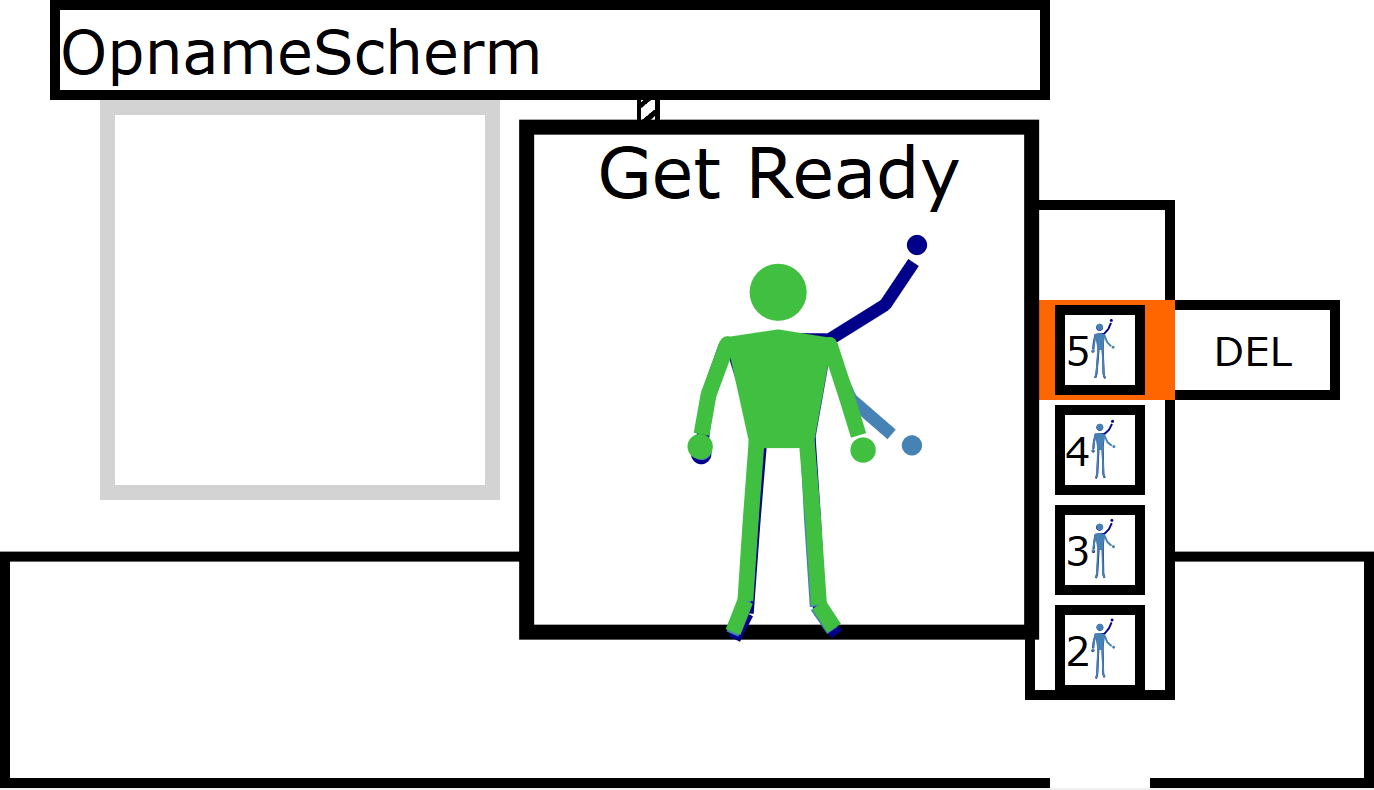
\includegraphics[width=12.5cm, height=7cm]{figures/4_record_getready.png}
		\caption{\emph{First view of the recording screen}}
		\label{first recording screen}
	\end{center}
\end{figure}

\begin{figure}[H]
	\begin{center}
		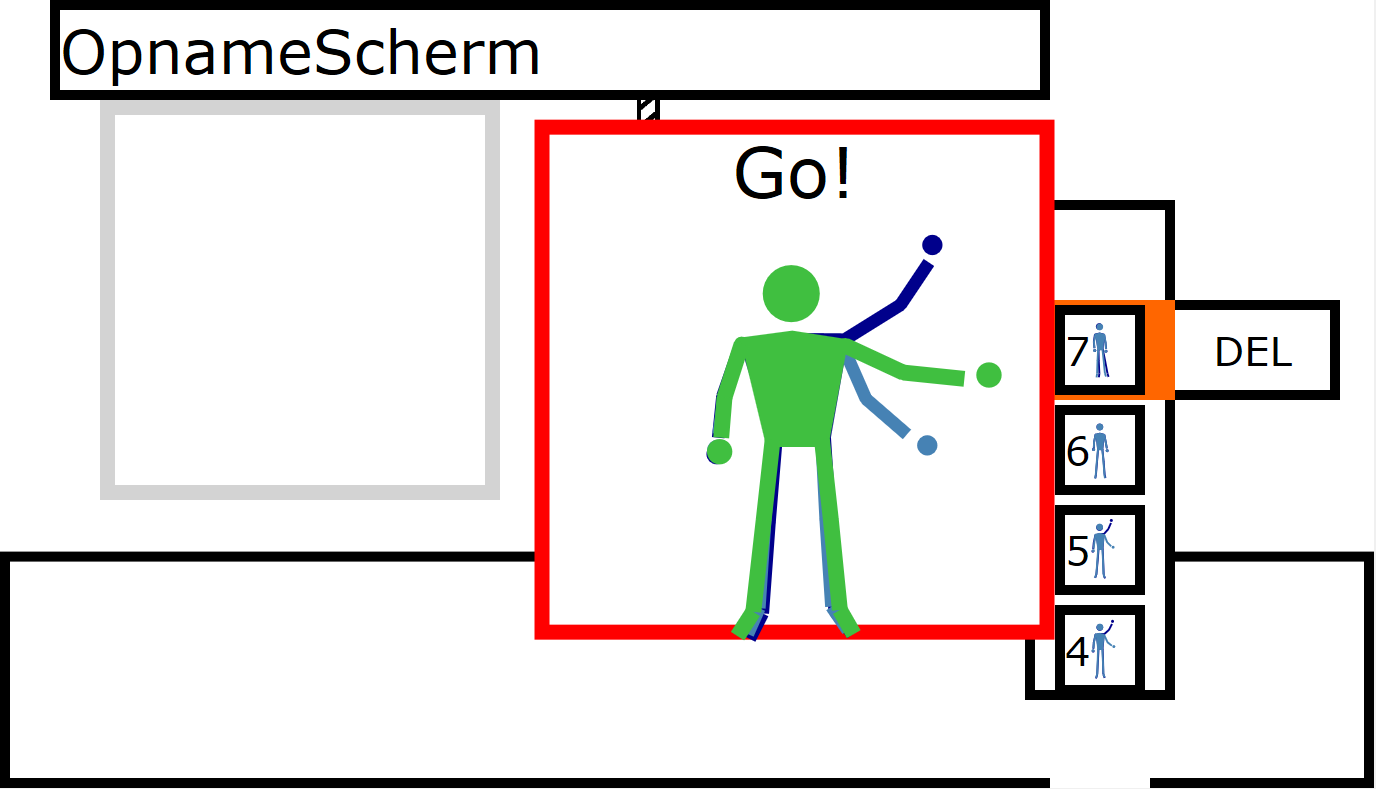
\includegraphics[width=12.5cm, height=7cm]{figures/6_record_start.png}
		\caption{\emph{View when the program starts recording, between this and the first view there is a countdown from 3, after the recording is started the user must stand still for a certain amount of time to stop, after which the text in the window will read "Done!"}}
		\label{last recording screen}
	\end{center}
\end{figure}

As described before, the scrollbar contains elements that are each linked to a recording of the current gesture. In these boxes a small preview can be seen of the start and end position of the linked recording in the same color scheme as during recording. The numbering of the boxes goes from the first recording as one counting up to the last recording. These numbers are not the same as the IDs of the gesture class as seen further on during the discussion of the implementation of the back end. The order of the numbers is still the same though. When the user hovers one of his hands over the recorded element within the orange selection box the effects as seen in \ref{replay of element six} are triggered. The specific recorded element is replayed within the previously grayed out window on the left. The blue bar on the bottom of the window indicates the progress in playing the recording. As long as the user hovers over the element in the scrollbar, the recording is repeated with half a second delays between repeats. This was a deliberate choice to make sure the user is fully aware of which recording is playing in the window because he should notice that the recording is only playing when he touches it. For the same reasons the number of the recording is also displayed on the left of the screen where it does not obstruct the user in reviewing his recording but is there when the user is uncertain of which recording is playing. Additionally both the orange selection box in the scrollbar and the edges of the display screen are colored green, the color previously linked with hover over information. The redundancy in linking the replay with the recording comes from the fact that the screen is so far from the actual element it is connected to. The scrollbar is on the right because right handed users are more common, so it is easier for them to operate the scrollbar. The delete action is already on the right of it and can hardly be moved to somewhere where it is still as easy to operate. Following both the proximity and similarity law of the Pragnanz law's would make the most sense but placing the screen on the right of the delete button would still have the delete button between it and the recorded element and would place the user's puppet too far from the center of the screen, out of the focus of the user.\\

\begin{figure}[H]
	\begin{center}
		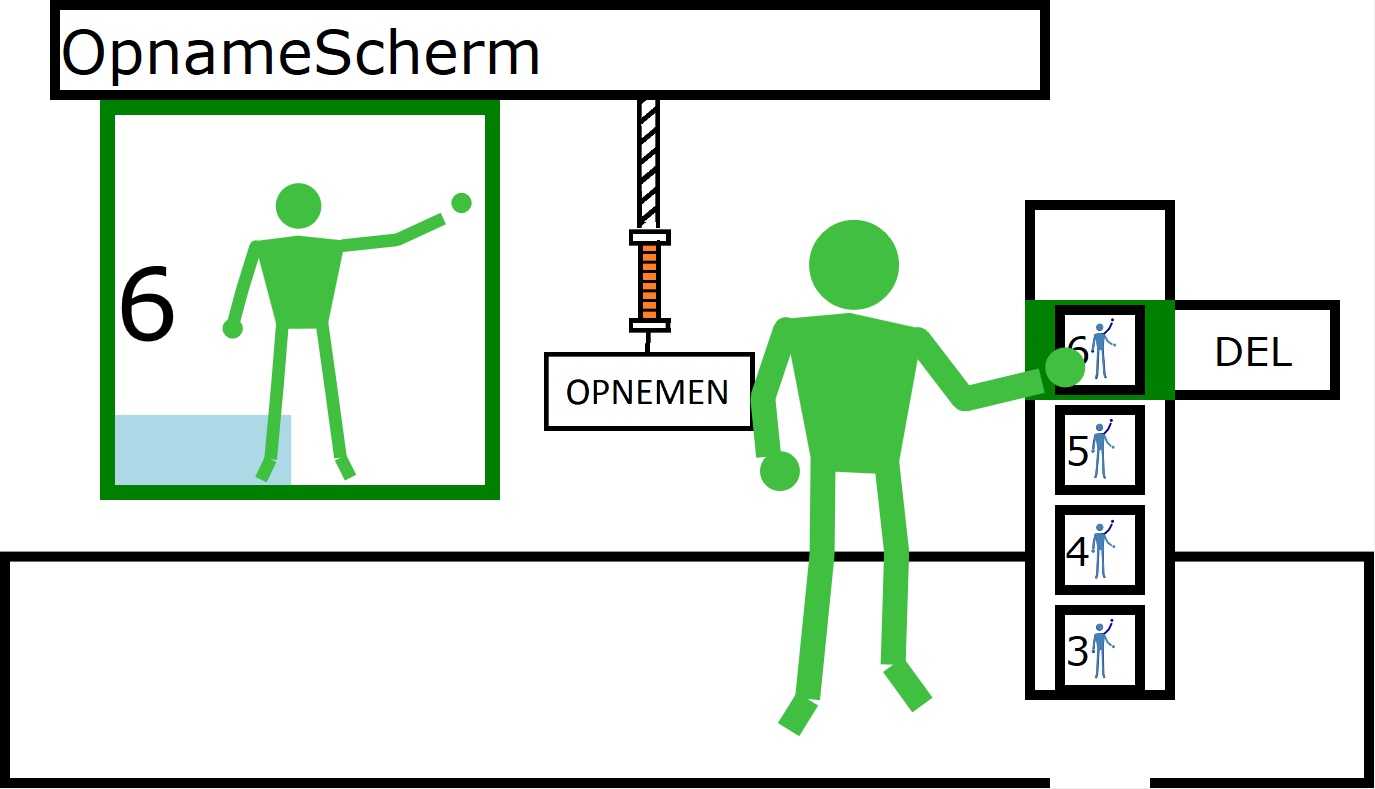
\includegraphics[width=12.5cm, height=7cm]{figures/11_replay_recording.png}
		\caption{\emph{The recorded element six is replayed to the user by hovering over it with any hand.}}
		\label{replay of element six}
	\end{center}
\end{figure}

To activate the scroll function on the scrollbar, the user has to hover his hand within the boundaries of the black bordered box but not within the orange selection box, the black borders of the scrollbar turn green to indicate that the user is hovering over the scrollbar, this is shown in figure \ref{scroll functionality} A. Scrolling only starts when the user has moved a small distance up or down to avoid to scrollbar being immediately stuck to the user which would be annoying. Once scrolling is started it continues as long as the user keeps moving in the same direction, this also counts when going through the selection box area and even when going outside of the scrollbar's borders. This makes sure that the user is not surprised by a sudden stop of the scrolling action when accidentally going inside of the selection box or outside of the scrollbar. The whole reason why the user cannot initiate a scroll within the selection box is because the element that is placed there has to be able to be hovered over to display it, as explained earlier, and it has to be able to be moved to the side for deletion. Accidental activation of the scroll function is minimized by this measure. Though there is more to this, informal tests showed that users who are unfamiliar with the UI often try to scroll down or upward starting from the selection box, the large delay in reaction confuses them. To counter this the activation area of the scroll function is expanded into the orange area for about 15 percent of the selection box height on both the top and the bottom. Once activated the elements stay on a fixed distance from each other but all elements are moved with the same dynamics as used in the record rope, they perform the same vertical relative movement as the hand that is hovering over it. During scrolling all recorded elements are locked to any interactions and the element that will land in the selection box is indicated by a light blue coloring of the white background. The example of scrolling can be seen in figure \ref{scroll functionality} B. When the user stops scrolling the recorded elements are locked into positions as seen in \ref{scroll functionality} A. Only the element in the selection box can be interacted with.\\

\begin{figure}[H]
	\begin{center}
		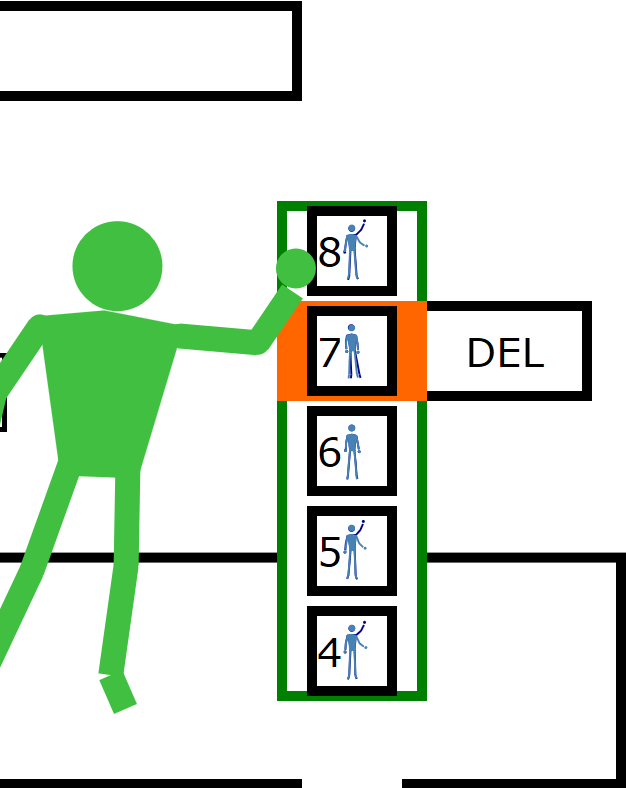
\includegraphics[width=6cm, height=8cm]{figures/9_hover_scrollbar.png}
		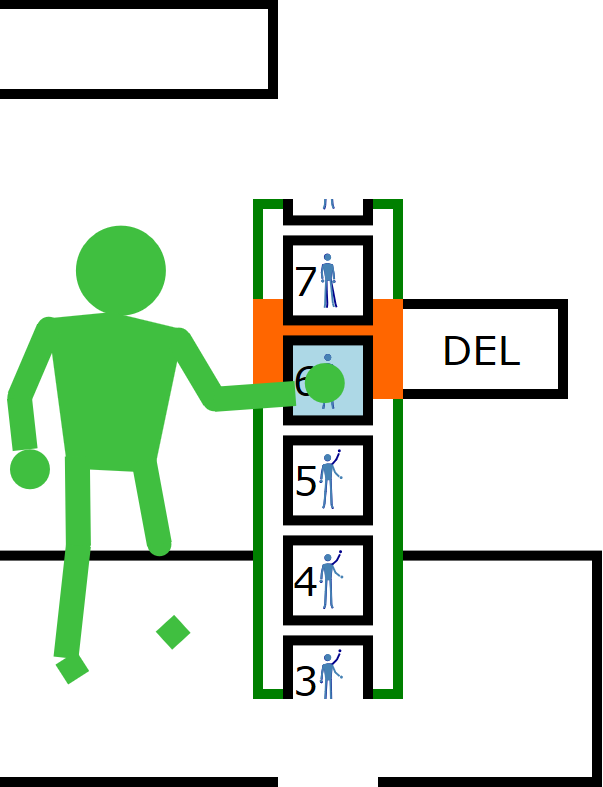
\includegraphics[width=6cm, height=8cm]{figures/10_scroll_scrollbar.png}
		\caption{\emph{Reaction of the scrollbar: A) when hovered over, B) when scrolling is activated}}
		\label{scroll functionality}
	\end{center}
\end{figure}

The delete sequence of the recorded element in the selection box can be started by hovering over the middle of it. After this the element will follow the relative horizontal movement of the interacting hand between start point and end point with the same dynamics as the scrollbar and the rope. As seen in figure \ref{delete functionality} A, The "DEL" box is filled up with a red progress bar to indicate how far the user still has to move until the item is deleted. When the end point is reached the recorded element turns red and fades away within a halve second to clearly indicate that this recording is deleted. Once the endpoint is reached the action is irreversible and for the duration of the fading the scrollbar and all the elements are locked for any further interaction. An example of this is shown in figure \ref{delete functionality} B. The reason why this action is only started from the middle is to increase the difference between initiating the delete sequence and replaying the recording and also heighten the threshold to start such a serious action as deleting an item. After deleting an element the other recorded elements are renumbered.\\

\begin{figure}[H]
	\begin{center}
		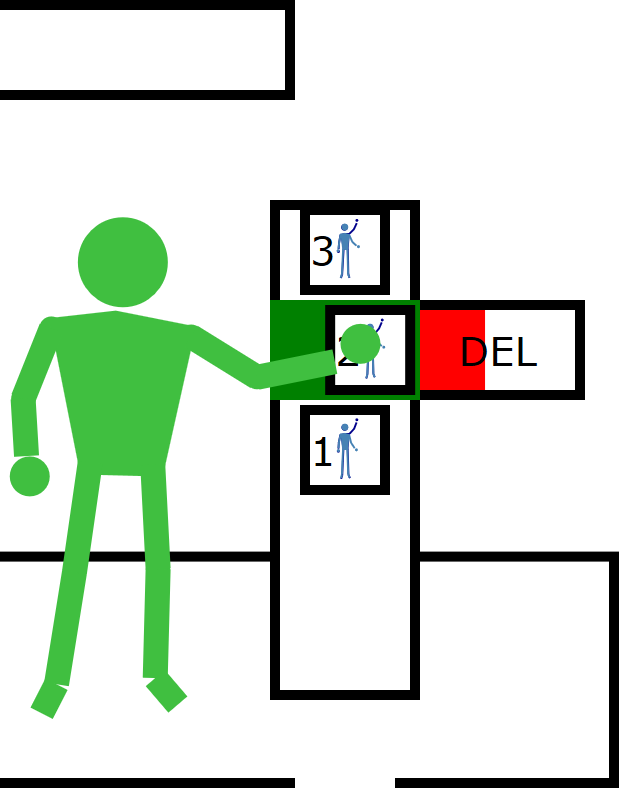
\includegraphics[width=6cm, height=8cm]{figures/12_delete_progress.png}
		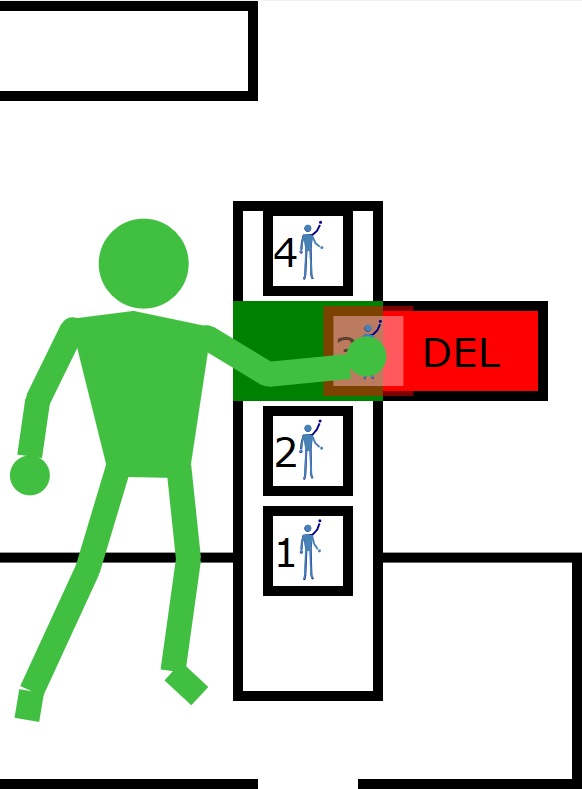
\includegraphics[width=6cm, height=8cm]{figures/13_delete_complete.png}
		\caption{\emph{The delete sequence: A) the user in the process of deleting, the red progress bar indicates how far until deletion the user has to go , B) The endpoint of the action is reached, the item turns red and fades after which it is deleted}}
		\label{delete functionality}
	\end{center}
\end{figure}


\section{Gesture recognition}

In order to provide enough flexibility concerning the type of gestures, SVM is used. SVM supports supervised machine learning and its use encompasses two modes: train and predict. After a discussion of the way SVM can be useful for this application, the approach relying on SVM to predict the executed gesture is explained.\\


\subsection{Support vector machine}

A model can be trained with a given data set and labels to classify each gesture. The data set contains all of the recordings of each gesture. A gesture consists of multiple recorded frames. Each frame is classified by using a label. This makes it possible to specify which frames belongs to a certain gesture. Each frame consists of 25 data points, called joints, which are measured by the Kinect camera. A single point is defined in 3D space, meaning that one frame is defined by 75 coordinates. In other words, one frame has 75 features and, as such, one frame can be seen as a single point in a 75-dimensional space.\\

It is possible to record the same gesture more than once and include all of these recordings in the data set. All recorded frames of the same gesture receive the same labels to indicate that they are basically the same gesture. While these gestures may appear to be identical, they contain slight variations due to noise during the measurement of a gesture or a slightly varying execution of the gesture by the user.\\

After performing all required gestures, a SVM model is created. Given a single frame of a gesture, this model can predict which of the recorded gestures the frame belongs to. SVM does this by finding the class of frames that are the most similar to the given frame and returns the label of that class as a result. This also implies the necessity of having multiple trainings recorded for each gesture. Errors in a single training due to noisy measurements of the Kinect camera can lead to wrong predictions. Having multiple trainings minimizes the influence noise has on the prediction and keeps into account that the user executes all gestures with slight variations. As a result, the model can predict more accurately which gesture is performed.\\

However, there are some things to keep in mind when applying this strategy. Firstly, inputting multiple repeats of the same gesture helps creating a better model, which improves predicting the gesture after a model is created. The downside is that it takes more time for the therapist to record all of these gestures. Secondly, when trying to predict a gesture, the generated SVM model always returns the label of the most similar gesture, even if they are not related at all.\\

These problems are tackled as part of the approach to using SVM to predict gestures. Also, the next section discusses how gesture recognition works for the OmniPlay application in more detail.


\subsection{Approach}

Two approaches are considered when it comes down to learning how to recognize gestures. By directly comparing these approaches, it is easier to identify their advantages and disadvantages.\\

The first approach is to add a time stamp to each frame as an extra feature, which indicates the time relative to the first frame of the gesture. This results in having 76 features per frame. The additional time stamp feature can be used to make sure that the gesture is not just similar in space, but also in time. If performing a certain gesture takes $t$ seconds and is captured at a rate of $f$ frames per second, this amounts to 76 $\cdot$$t \cdot f$ features. For a 4-second gesture recorded at 30 frames per second, which is the highest sampling speed of the Kinect camera, this amounts to 9120 features for a single training of the gesture. In other words, the number of features of one training depends on the duration of the gesture. The entire gesture is classified as a single gesture. During prediction, a gesture with the same number of features can be input. As a result, SVM returns the class of gestures that is the most similar to the given gesture.\\

There are several problems with this first approach. If the number of features of the gesture used for predicting does not match the number of features of the training gestures, the prediction is not accurate and should be discarded. Discarding is necessary as SVM always returns the label of a gesture, even if the predicted gesture is completely unrelated to any of the gestures used for training the model. This poses a problem as different gestures can have a different duration. Even different recordings of the same gesture can take for instance 4 seconds and 4.1 seconds, implying that they have a different number of frames and thus a different number of features. A possible solution is to recalculate the entire gesture and use interpolation to convert the set of frames to a new set with a known, fixed size and preferably with equidistant time stamps. Using time stamps also implies that it is necessary to know when exactly a gesture starts and ends.\\

Furthermore, not just the different recordings of one gesture, but all of the gestures need to have the same number of frames. The gesture to predict is not known beforehand and can only be predicted accurately if the number of features for both the predicted gesture and trained gesture are equal. As a result, it is required that all gestures have an equal amount of features. This means that short gestures need to be mathematically extended with additional frames to match the size of longer gestures. Another side effect is that all gestures need to have the same duration, not just the same amount of features. This limits the therapist in choosing exactly what gestures he wants the patient to perform. Because of this, the action of predicting a gesture can only start when enough time has passed for the player to perform the gesture with the longest duration. More in particular, assume the longest gesture is 5 seconds in length. It then follows that it takes about 5 seconds to predict any gesture. This also means that patients that control the game can only perform one action every 5 seconds. As the games to be played are unknown beforehand, a slow reaction time of the application can render some games unplayable. As such, this approach is not viable.\\

The second approach is to split up one gesture into $n$ smaller gestures and classify each of them differently, assigning a different label to each part of the gesture. Assume that a gesture is split up into 4 smaller parts so that each part contains approximately an equal amount of frames (see figure \ref{fig: gesture_split}). Consider a 4-second gesture sampled at 30 frames per second. The complete gesture consists of 120 frames. By splitting it up into 4 parts, each part contains 30 frames. All first 30 frames are labeled with the same label, for instance 1. The next 30 frames receive a label 2, and so on. In other words, the considered gesture is split up into 4 postures with each having 30 slightly varying trainings. In contrast to the first approach, as described above, prediction does not happen for an entire gesture, but for separate postures. The condition for having executed the entire gesture is that each of the postures are predicted correctly and in the right order. To put it differently, $n$ \emph{pictures} are taken of the gesture and if at some point during prediction all pictures are executed in the right order, the application acknowledges the execution of the gesture.\\

\begin{figure}[H]
\begin{center}
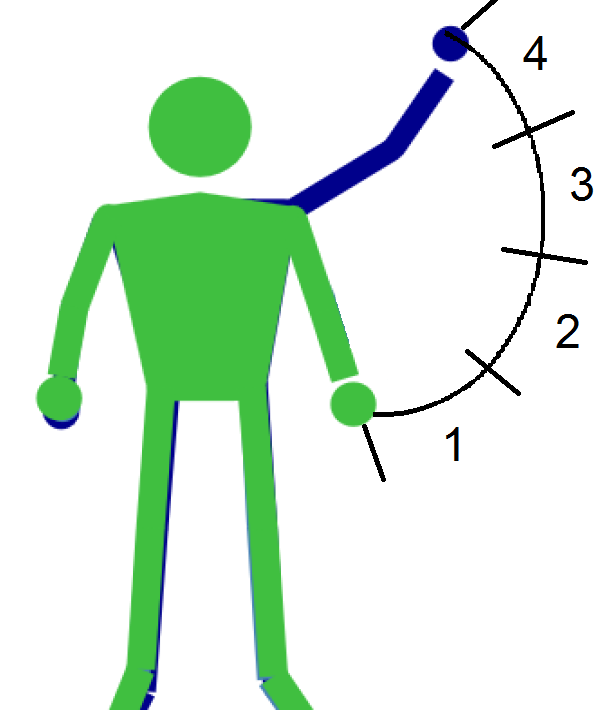
\includegraphics[width=5cm]{SVMGesture.png}
\caption{\emph{An executed gesture, split up into four parts}}
\label{fig: gesture_split}
\end{center}
\end{figure}

The biggest advantage of this approach is the flexibility of it. Each posture corresponds to a single frame, which contains 75 features. This eliminates the need of having gestures with the same length or having to modify training data to have gestures with an equal number of features. It is even possible to not just link a gesture, but also a posture to a virtual keyboard button, which allows the physical therapist to choose the gestures that fit the needs of a patient the best. Additionally, the application reacts immediately to an executed gesture, not after a fixed amount of time. This allows for a wider variety of games being playable using this application.\\

Another advantage is that it solves the issue where SVM always returns the label of a predicted gesture class, even when the patient is not doing anything. A gesture is only recognized when all parts of it are executed. In other words, gestures are not recognized involuntarily and, as such, actions like button presses that influence the game are not executed by accident.\\

A limitation of this second approach is that the physical therapist has no way to choose how fast the patient should perform a gesture. There is no strict requirement for the entire gesture to be executed in about the same time as the recorded gesture used to train the SVM model. If a gesture is executed faster during prediction compared to during training, it is recognized as the same gesture being executed. However, it is possible to solve this timing issue to some extent when the gesture during predicting is performed slower. The gesture can be ignored if more than a certain amount of time passes. This time threshold takes the gesture with the longest duration into account and is chosen higher than this in order to allow all gestures to be executed and successfully recognized.